%% Copernicus Publications Manuscript Preparation Template for LaTeX Submissions
%% ---------------------------------
%% This template should be used for copernicus.cls
%% The class file and some style files are bundled in the Copernicus Latex Package, which can be downloaded from the different journal webpages.
%% For further assistance please contact Copernicus Publications at: production@copernicus.org
%% https://publications.copernicus.org/for_authors/manuscript_preparation.html


%% Please use the following documentclass and journal abbreviations for preprints and final revised papers.

%% 2-column papers and preprints
\documentclass[acp, manuscript, english]{copernicus}

\begin{document}

\title{Toward non-hydrodynamic simulation of moist convection}


% \Author[affil]{given_name}{surname}

\Author[1]{DeWitt}{Thomas}
\Author[]{}{}
\Author[]{}{}

\affil[]{University of Utah}
\affil[]{ADDRESS}

%% The [] brackets identify the author with the corresponding affiliation. 1, 2, 3, etc. should be inserted.

%% If an author is deceased, please mark the respective author name(s) with a dagger, e.g. "\Author[2,$\dag$]{Anton}{Smith}", and add a further "\affil[$\dag$]{deceased, 1 July 2019}".

%% If authors contributed equally, please mark the respective author names with an asterisk, e.g. "\Author[2,*]{Anton}{Smith}" and "\Author[3,*]{Bradley}{Miller}" and add a further affiliation: "\affil[*]{These authors contributed equally to this work.}".


\correspondence{NAME (EMAIL)}

\runningtitle{t}

\runningauthor{TEXT}





\received{}
\pubdiscuss{} %% only important for two-stage journals
\revised{}
\accepted{}
\published{}

%% These dates will be inserted by Copernicus Publications during the typesetting process.


\firstpage{1}

\maketitle



\begin{abstract}
TEXT
\end{abstract}


\copyrightstatement{TEXT} %% This section is optional and can be used for copyright transfers.


\introduction  %% \introduction[modified heading if necessary]

The cloud feedback remains the most uncertain component of Earth's climate sensitivity, partly due to the fact that important physical processes span a very wide range of spatial scales. The default assumption is that increasing model resolution will reduce uncertainty \citep{shukla2009, slingo2022}, although ever-larger simulations built over the past 40 years have yet to reduce model spread in estimates of either the cloud radiative feedback \citep{ipcc6,ceppi2017} or the overall climate sensitivity (cite). % https://www.science.org/doi/10.1126/sciadv.aba1981 

It is argued that the next generation of kilometer-scale models will break the trend because they can resolve individual clouds \citep{slingo2022}. The implicit assumption is that clouds are typically kilometer-scale such that they may be resolved by kilometer-scale grid spacings. The ubiquity of this assumption is exemplified by the equivalent terminology ``Global Cloud-Resolving Models'' (GCRMs). However, the assumption that cloud dynamics are kilometer scale appears contradicted by the property of scale invariance in cloud shapes and sizes, which has been observed to apply globally from subkilometer scales up to thousands of kilometers \citep{wood2011,guillaume2018,dewitt2024,rees2024,dewitt2024b,dewitt2026}. Scale invariance implies that kilometer scales are no more fundamental than any other scale within the invariant regime: kilometer-scale phenomena are simply a rescaled version of 100-kilometer-scale phenomena without being qualitatively different \citep{lovejoy2013}. The implication would be that a physically accurate cloud parameterization should, in principle, work equally well in a 100-kilometer simulation as a 1-kilometer simulation. Conceivably, then, the reason the cloud feedback is uncertain is not that the models have insufficient resolution but rather that our parameterizations for clouds are insufficient. 


On a fundamental level, any parameterization is equivalent to a theory for cloud dynamics, as both attempt to represent a more complex phenomenon through simpler means \citep{arakawa2004}. This could be viewed as analogous to how the Navier-Stokes equations themselves represent a substantial simplification over a particle-by-particle accounting of the same system. This is a phenomenon referred to as ``emergence'', where some simplified set of laws can still describe many important features of a complex system, and without needing to explicitely simulate every smaller-scale detail. Just as the Navier-Stokes ``emerge'' out of a sufficiently complex collection of particles, a hypothetical theory for cloud dynamics might ``emerge'' out of a sufficiently complex turbulent flow. That parameterizations work at all suggests that such an emergent theory may exist, even if it is not yet understood.

At the root of the problem of the cloud radiative effect, then, is a theoretical problem: how can the extreme complexity of a cloud field be represented in some simplified state space, using some set of emergent laws? How can the dynamics at one scale, such as those resolved in a GCM, be related to the dynamics at other scales, such as those being parameterized? Although these questions may be quite difficult to answer in any sufficiently general way, we have no choice but to attempt an answer. Parameterizations must be used whether or not they have a plausible physical foundation.

There is a long history of analytical forumlations of clouds and cloud fields in terms of a large number of constituent elements, even if what serves as the basic element is not yet agreed upon. An early example is \cite{arakawa1974}, who derived a convective parameterization by modeling individual clouds as convective "plumes" using similarity theory. However, given that plumes require a constant source of buoyancy, their applicability to moist convection has been called into question. Instead, thermals or ``bubbles'' have been proposed as a better starting point for a similarity theory-based cloud model (yano), suggesting cloud fields may be thought of as a large number of superimposed thermals.
Other work has attempted to take clouds themselves as the basic constituent element in order to derive overall statisics of fields containing large numbers of clouds \citep{craig2006, cohen2006, garrett2018}. Unforuntately, even individual clouds are highly complex structures, and cloud theories therefore tend to make major simplifications such as ignoring interactions between clouds \citep{craig2006} or making clouds binary objects \citep{garrett2018}. 

Although it is less commonly applied to clouds, a much older tradition exists of conceptualizing fluid flows as being made up of constituent parts: a turbulent cascade. As first articulated by (Richardson), here a turbulent flow is envisioned to be made up of large numbers of ``eddies'' that recursively break up into smaller and smaller eddies through a ``cascade'' while conserving some relevant physical quanitity such as the kinetic energy dissipation rate. 

Despite being widespread in turbulence theory, the cascade is typically only invoked as a conceptual argument used to motivate scaling arguments such as the Kolmogorov -5/3 energy spectrum, where kinetic energy $E$ is related to wavenumber through $E\propto k^{-5/3}$. It is rarely taken as a literal description of the dynamics that could be used to make simulations. Multiplicative cascades are a partial exception, but even here eddies are difficult to interpret as physical constituents of the flow, and the most realistic simulation methods substitute a cascade for more physically opaque mathematical methods \citep{lovejoy1990,lovejoy2010FIF}.

Conceptually, eddies and bubbles bear some resemblance insofar as both form the consituent elements from which the overall field is built. However, turbulence and the dynamics shaping clouds are typically thought to be distinct physical processes operating at different spatial scales, primarily because buoyancy is central to cloud dynamics but is omitted from Kolmogorov's theory of turbulence. It is therefore understandable that bubbles and eddies have thus far been considered separately. However, what is less widely recognized is that buoyancy may be incorporated into the theory of turbulence itself, in which case the concepts of eddies and bubbles might be unified to construct a theory of cloud dynamics. 

As suggested by \citet{schertzer1985}, when buoyancy is present in a turbulent flow, it is not kinetic energy flux that is conserved through the cascade, but a different flux related to buoyancy. The reason is that kinetic energy may be converted into potential energy in a gravitational field and is therefore not conserved. The main empirical consequence of ``Lovejoy-Schertzer'' turbulence is that Kolmogorov's -5/3 energy cascade only applies when the power spectrum is computed along the horizontal direction: $E\propto k_x^{-5/3}$. When computed along the vertical, a different relationship was proposed, namely $E\propto k_z^{-11/5}$. This directional dependence of the kinetic energy spectrum was recently found to be closely consistent with sonde observations and LES output from scales of 200 m to 2000 km. These scales include nearly the full range of motions that are typically associated with cloud dynamics, suggesting that ``bubbles'' may indeed be equivalent to ``eddies'' -- so long as the theory of turbulence considered is that proposed by Lovejoy and Schertzer, not Kolmogorov.

Here, we propose a model for clouds by formalizing the conceptual model of a Lovejoy-Schertzer turbulent cascade in a physically realistic manner. The model is based on the idea that a cloudy turbulent flow can be thought of as being composed of a large number of discrete constituents, which we refer to as ``turbulons''. A turbulon is like an ``eddy'' or ``bubble'' but has a specific mathematical form and applies to an arbitrary vector or scalar field. We propose an algorithm that may be used to simulate three-dimensional volumes of water vapor and condensate, temperature, and moist static energy using turbulons, called the Superposition of Turbulon and Eddy Atmospheric Model (STEAM). Renderings of the generated cloud fields using a ray-tracing algorithm display striking realism (Fig. ), suggesting the model may pass the ``Palmer-Turing test'' for visual fidelity \citep{palmer2016,christensen2021}. We show quantitatively in Sect. (REF) that many aspects of STEAM-simulated fields are comparable to state-of-the-art high-resolution hydrodynamic models, although not in every case. Some differences between STEAM and the hydrodynamic benchmark suggest concrete steps for future work, while others are more mysterious. Conceivably, some discrepancies may even indicate STEAM is more realistic than the hydrodynamic comparison: using a comparison to MODIS satellite observations in Sect. (REF), we show that STEAM reproduces several statistics describing cloud geometry more accurately than the hydrodynamic baseline. We rigorously estimate STEAM's computational advantage over a comparable hydrodynamic model to be NUMBER on the same hardware.

\section{Theoretical basis for STEAM}

In this section, we provide a high-level overview of the theoretical considerations used to formulate the Superposition of Turbulon and Eddy Atmospheric Model (STEAM). A complete description of the STEAM algorithm is provided in Appendix \ref{sect:steam algorithm details}.

The basic idea of a turbulent cascade is to consider the fluid volume as being made up of a discrete set of constituent elements called ``eddies'', i.e. circulations in the wind field. In order to formalize this idea, we must first specify exactly what we mean by a turbulent eddy and extend the concept to fields other than the wind field. In place of the term ``eddy'', we introduce the term ``turbulon'' to refer to an individual constituent element of a turbulent field (Fig. \ref{fig:turbulon concept}). A turbulon $\mathfrak{t}$ is defined as a set of localized perturbations in all fields that make up a turbulent flow. Perturbations in each field have an identical shape but varying amplitude. For example, a given turbulon might be associated with a strong temperature perturbation but a weak pressure perturbation. The turbulon shape is defined by some ``envelope'' function $\mathfrak{T} (\ell, \mathbf{r})$ with size parameter $\ell$. Any individual turbulon is made up of components that are a scaled and translated version of the envelope function with a specified size parameter $\mathfrak{t}_i = a(\mathbf{r}, \ell)\mathfrak{T}(\ell, \mathbf{r} - \mathbf{r}')$, where $a$ is the perturbation amplitude. Conceptually, turbulons are broader than the concept of ``eddies'' and more precise. Eddies are rarely defined mathematically, but if they were, an eddy would only represent the component of a turbulon that is associated with a perturbation in the wind field.

\begin{figure*}[t]
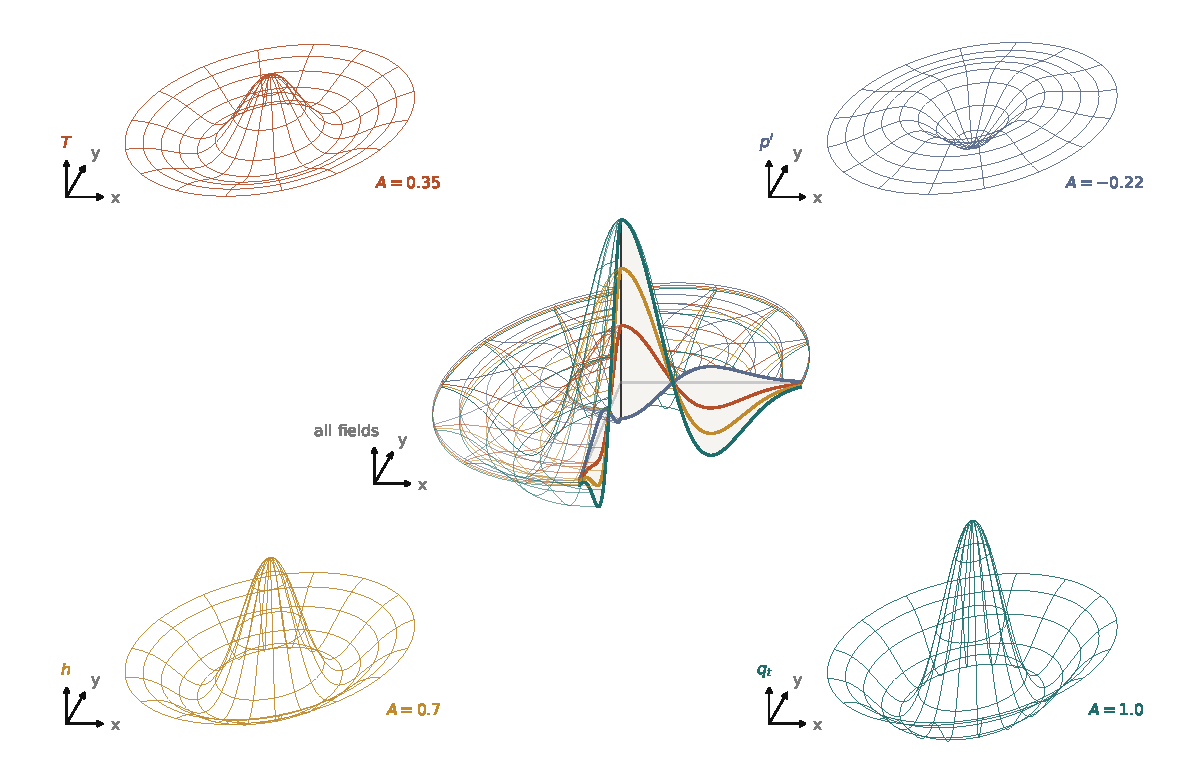
\includegraphics[width=12cm]{concept-figs/w7_quincunx_asym.pdf}
\caption{A single two-dimensional ``turbulon'': a set of localized perturbations in each field from which a turbulent field is built. Each perturbation (corners) associated with a single turbulon $\mathfrak{t}$ (center) has a varying amplitude $A$ but a common shape, defined by the envelope function $\mathfrak{T}$, here a two-dimensional Mexican Hat analogous to that used for STEAM (Eqn. \ref{apxeq:turbulon shape}).} \label{fig:turbulon concept}
\end{figure*}

The overall field $F$ defining a component of the atmospheric state, perhaps representing temperature or moist static energy, is represented as a superposition of a large number of turbulon components as shown in Fig. \ref{fig:field superposition}:
\begin{align}
  F(\mathbf{r}) = \sum_{\ell, \mathbf{r}'}^{} a(\mathbf{r}, \ell)\mathfrak{T}(\ell, \mathbf{r} - \mathbf{r}'). \label{eq:basic field construction with turbulons}
\end{align}

\begin{figure*}[t]
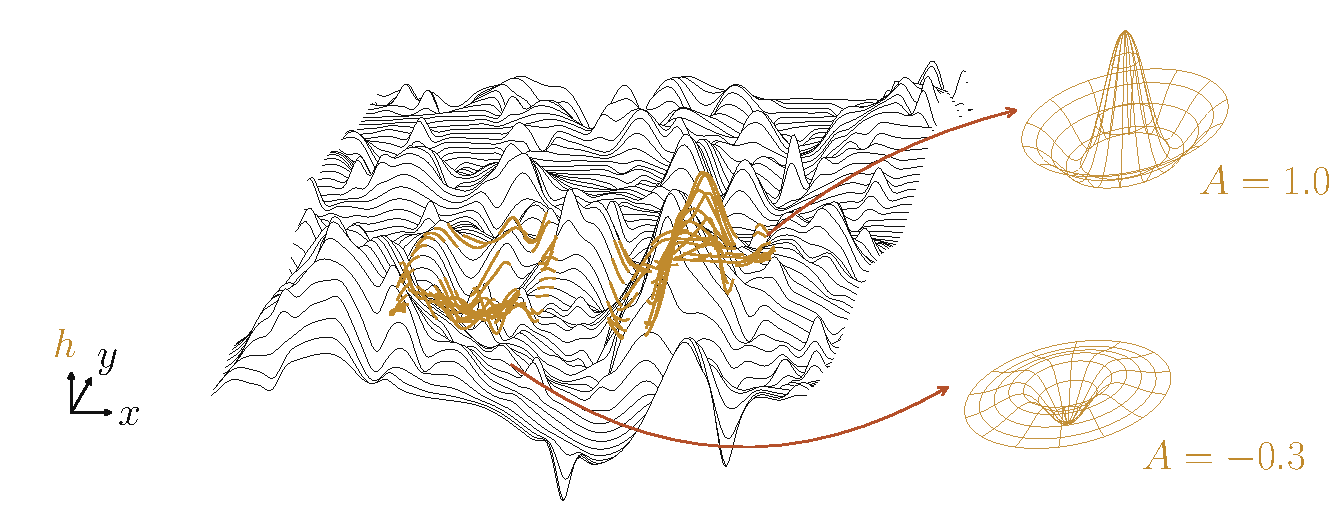
\includegraphics[width=12cm]{concept-figs/v11c_field_h.pdf}
\caption{A two-dimensional turbulent field of moist static energy $h$ (left) is built from a superposition of a large number of individual turbulons with varying amplitudes and positions (Eqn. \ref{eq:basic field construction with turbulons}). Shown on the right are the $h$-component of two such turbulons.} \label{fig:field superposition}
\end{figure*}


Mathematically, the approach is equivalent to a wavelet transform, a method already common in turbulence theory and discussed further below. However, almost exclusively wavelets are used as an analysis tool to determine how much variance a given signal has as a function of location and frequency. We are proposing to invert this interpretation: given sufficient theoretical constraints on the statistics of the turbulons, the wavelet formalism may not only be used to analyze atmospheric volumes but also to simulate them. More fundamentally, we also propose an ontological re-evaluation of wavelets as more than just a mathematical tool used to evalute frequency content. In this conception, a cloud is made up of constituent elements called turbulons, in the same way that an ideal gas is made up of particles. This conceptual shift can provide a new and complimentary perspective on atmospheric turbulence and cloud dynamics.

The wavelet equivalence implies that any possible field $F$ may be simulated given the correct turbulon statistics using Eqn. \ref{eq:basic field construction with turbulons}. Therefore, any given question of atmospheric statistics or dynamics posed in real space has an equivalent formulation in the ``turbulon space'' represented by the turbulon amplitudes and locations $a_i(\mathbf{r},\ell)$. As clouds and turbulence are inherently multi-scale phenomena, turbulon space has the benefit of explicit separation as a function of the scale parameter $\ell$. And as we will now show, turbulence theory provides several important constraints on the statistics of the turbulons as a function of the size parameter $\ell$.

Most commonly, theories of turbulence provide a constraint on the kinetic energy spectrum of some component of the wind field $v$. This constraint on the frequency content may be represented in either wavenumber space, using the spectrum, or real space, using wavelets or, more commonly, structure functions. The structure function is defined as 
\begin{align}
  \Delta v (r)\equiv \big|v(\mathbf{x})-v(\mathbf{x}+\mathbf{r})\big|; \qquad r \equiv |\mathbf{r}|,
\end{align}

% Note that there are multiple choices for the allowed directions of the separation vector $\mathbf{r}$. For Kolmogorov turbulence, isotropy implies that all directions have identical statistics.
Turbulence theories typically constrain how the mean amplitude of the structure function scale with the separation vector $r$ by raising $\Delta v$ to some power $q$ and then ensemble averaging over many spatial locations $\mathbf{x}$ to obtain $\langle \Delta v (r)^q\rangle$.
If the kinetic energy spectrum follows a power law $E\propto k^{-\beta}$, the second-order structure function with $q=2$ scales as \begin{align}
  \langle\Delta v^2 (r)\rangle\propto r^{\xi(2)}\qquad \xi(2) = \beta - 1. \label{eq:isotropic KE structure function}
\end{align}
For the homogenous isotropic turbulence considered by Kolmogorov, $\beta =5/3$.
One advantage of the structure function is that, unlike the spectrum, structure functions may be defined for arbitrary orders $q$. This propoerty becomes useful when the flow becomes ``intermittent'' and the strongest fluid gradients become clustered spatially rather than evenly distributed. The strength and character of turbulent intermittency can be quantified via the function $\xi(q)$ as we show in Sect. (). 

Atmospheric turbulence does not in general follow the isotropic law (Eqn. \ref{eq:isotropic KE structure function}) due to the effects of buoyancy. A more accurate description of atmospheric flow is ``Lovejoy-Schertzer'' turbulence, where structure functions for horizontal wind components are a function of separation direction as well as distance. The reason for the directional separation is that only vertical motions are affected by gravity, and so the quantity controlling the turbulent cascade along the vertical direction is related to buoyancy. In contrast, the horizontal component of the cascade is not affected by buoyancy and therefore structure functions follow the Kolmogorov law when calculated along a purely horizontal direction. \citet{lovejoy1985} proposed that structure functions should follow
\begin{align}
  \begin{cases}
    \langle\Delta v (\Delta x)\rangle = \varepsilon^{1/3} r^{H_h}; \qquad H_h=1/3; \qquad \Delta x \equiv |\mathbf{r}(\Delta x, \Delta z=0)|\\
      \langle\Delta v (\Delta z)\rangle = \phi^{1/5} r^{H_v}; \qquad H_v=3/5;\qquad \Delta z \equiv |\mathbf{r}(\Delta x=0, \Delta z)| 
\end{cases}\label{eq:LS directional structure functions}
\end{align} 
where $H_h$ and $H_v$ are called Hurst exponents for horizontal and vertical separations, respectively. The proportionality constant $\varepsilon$ represents Kolmogorov's ``kinetic energy flux'', i.e. the rate of kinetic energy transfer from large to small scales $\partial v^2/\partial t$. The quantity $\phi=\partial f^2/\partial t$, called ``buoyancy variance flux'', is also a down-cascade variance flux analogous to kinetic energy but for buoyancy $f$. Equation \ref{eq:LS directional structure functions} was proposed as a conjecture that combined two isotropic theories, namely by Kolmogorov and Bolgiano-Obukhov into the anisotropic form represented by Eqn. \ref{eq:LS directional structure functions}. Whether or not the fluxes $\varepsilon$ and $\phi$ may be interpreted the same way in the isotropic and anisotropic forms is an open question \citep{dewitt2025bpreprint}. 

Regardless of the exact physical interpretation, the predicted Hurst exponent values in Eqns. \ref{eq:LS directional structure functions} have recently been shown to agree closely with global dropsonde and datasets and LES simulations \citep{dewitt2025bpreprint}. For horizontal wind components, $H_v\approx 0.7$ when computed along the vertical direction for separations between $200\,\unit{m}$ and $7\,\unit{km}$, whereas $H_h\approx 0.4$ for structure functions computed along the horizontal direction for separations between $200\,\unit{m}$ and $2000\,\unit{km}$. Both values are nearly consistent with Lovejoy-Schertzer turbulence while also ruling out the alternatives such as isotropic Kolmogorv turbulence or quasi-geostrophic turbulence over the observed range. Thus, although turbulence is often thought to be a small-scale phenomenon, if it is considered using Lovejoy-Schertzer theory rather than Kolmogorov theory, a very wide range of scales can be said to be turbulent including almost all scales relevant to cloud dynamics.

Given that the wind field transports numerous other quantities, the value of the Hurst exponent for wind affects the Hurst exponents for other variables, including any conserved advected scalar $\Phi$ following
\begin{align}
  \frac{D\Phi}{Dt} = 0.\label{eq:advection conservation}
\end{align} 
For simulations, below we will take $\Phi$ to be equal to moist static energy and total water content, but other conserved scalars could be simulated as well. 
In general, Hurst exponents for $\Phi$ are thought to be equal to the Hurst exponents for the wind field \citep{lovejoy2013}. In classical isotropic turbulence theory, the Hurst exponent is $1/3$, a result known as the Corrsin-Obukhov law of scalar advection. For Lovejoy-Schertzer turbulence, the analogous law is 
\begin{align}
  \begin{cases}
  \langle\Delta \Phi (x)\rangle\propto \langle |x|^{H_x}\rangle; \qquad H_x=1/3, \\
  \langle\Delta \Phi (z)\rangle \propto \langle |z|^{H_v}\rangle; \qquad H_v=3/5,
  \end{cases}\label{eq:LS scalar directional structure functions}
\end{align}
where $H_x$ and $H_v$ are equal to their values for the horizontal component of the wind field (Eqn. \ref{eq:LS directional structure functions}). Observationally, \citet{lilley2004} found Hurst exponents for the aerosol backscatter ratio of $H_h=0.33\pm0.03$ and $H_v=0.60\pm0.04$, in excellent agreement with Eqn \ref{eq:LS scalar directional structure functions}. 

Hurst exponents for quantities that are not pure advected scalars might not follow Eqns. \ref{eq:LS scalar directional structure functions}, but the turbulon picture suggests perturbations could still be expected to display the aspect ratio scaling prescribed by Eqn. \ref{eq:turbulon aspect ratio scaling}, given that the perturbation shape is shared across fields for a given turbulon while the amplitude is not. Indeed, \citet{guillaume2018} found that the aspect ratio of cloud cross-sections, as observed by the CloudSat satellite-based radar, show the predicted aspect ratio scaling, although their reported results require some algebraic manipulation as we show in Appendix \ref{sec:guillame}.


\subsection{Distribution of turbulon amplitudes across scale} \label{sect:distribution of turbulon amplitudes across scale}

Both structure functions and wavenumber spectra represent a scale decomposition of a signal, where scale is measured using either field differences or wavenumber. Both may be recast as a special case of a generalized scale decomposition framework using wavelet transforms. Here, this framework is useful because it shows that the differences in Eqn. \ref{eq:LS directional structure functions} may be replaced by a turbulon envelope function $\mathfrak{T}$ without any change to the power-law dependence in $\Delta x$ or $\Delta z$. Thus, Eqn. \ref{eq:LS directional structure functions} may be interpreted as a constraint on the mean absolute amplitude of the turbulons as a function of their scale parameter $\ell$. Specifically, if the turbulon envelope function is defined through

(eqn, deltas, etc)


then the structure function may be equivalently defined through a convolution 
\begin{align}
\langle \Delta f^q\rangle(\ell) = \langle\left(\big|\mathfrak{T}(\ell) * f\big|\right)^q\rangle_r\label{eq:wavelet transform}
\end{align}
where the operator $\langle\rangle_r$ represents an average over all spatial locations $r$. If, for each $q$, the structure function Eqn. \ref{eq:wavelet transform} follows a power law in $\ell$, there are other choices of the turbulon envelope function $\mathfrak{T}$ that result in an identical power-law exponent, at least over the range where discretization effects can be neglected. Equation \ref{eq:wavelet transform} therefore represents a generalization of the structure function which we refer to as a ``fluctuation function.'' Where discretization effects dominate, different choices of $\mathfrak{T}$ do affect the power-law exponent. For example, Figure () shows the mean wavelet transform ($q=1$) for a random walk, for three common choices of $\mathfrak{T}$ defined through a structure function, a Mexican hat, and a Haar wavelet. For each function, a local power law exponent is computed as $d\log \langle \Delta f^q\rangle/d\log \ell$ and shown in Panel (). This local power-law exponent represents the Hurst exponent at each scale $\ell$, and it attains its theoretical value of 0.5 only above $\ell\gtrsim ?$. The consequence is that the choice of the turbulon envelope function does not affect the resulting two-point statistics, but only at scales much larger than the grid scale, and that such discretization effects are not a specific limitation of the model but a general feature of discretization. The only limitation on the shape of $\mathfrak{T}$ is the admissability criterion for discretized wavelets: namely, that they have zero mean.

The anisotropy implied by Eqn \ref{eq:LS directional structure functions} -- where the Hurst exponent is a function of direction -- is also straightforward to model, simply by allowing the turbulon aspect ratio to vary as a function of the turbulon size (Fig. \ref{fig:cascade slice}). Using $H_z=5/9$, the turbulon aspect ratio therefore follows
\begin{align}
  \frac{\ell_z}{\ell} = \ell_s^{4/9} \ell^{-4/9}\label{eq:turbulon aspect ratio scaling}
\end{align}
where $\ell$ and $\ell_z$ are the horizontal and vertical size parameters of the turbulons, respectively.
The proportionality constant $\ell_s$ is termed the ``spheroscale'' and defines the scale at which the aspect ratio becomes 1, i.e. where $\ell=\ell_z=\ell_s$. Scales smaller than the spheroscale have yet to be observationally evaluated within the LS framework. Based on visualizations of STEAM simulations discussed in Sect. (), we conjecture that isotropic Kolmogorov turbulence is recovered below the spheroscale, but it could also be possible that the anisotropy specified by \ref{eq:turbulon aspect ratio scaling} persists, implying that turbulons become vertically elongated and pill-shaped at small scales. Regardless, $\ell_s$ tends to be of order 1 to 10$\,\unit{m}$, and so isotropic turbulence only exists at very small scales if at all.

The aspect ratios prescribed by Eqn. \ref{eq:turbulon aspect ratio scaling} are also consistent with Eqn. \ref{eq:LS directional structure functions}. Specifically, simulations set the mean absolute turbulon amplitude such that 
\begin{align}
  \langle |\mathfrak{t}|\rangle \propto \ell^{H_h} .\label{eq:turbulon amplitude vs scale}
\end{align} 
If $\ell$ is related to the vertical size parameter $\ell_z$ through
$  \ell^{H_z}\propto \ell_z, $
then $\langle |\mathfrak{t}|\rangle \propto \left(\ell_z^{1/H_z}\right)^{H_h}=\ell_z^{H_h/H_z}$. If $H_z=5/9$, we obtain the vertical dependence specified by Eqn. \ref{eq:LS directional structure functions}.


\begin{figure*}[t]
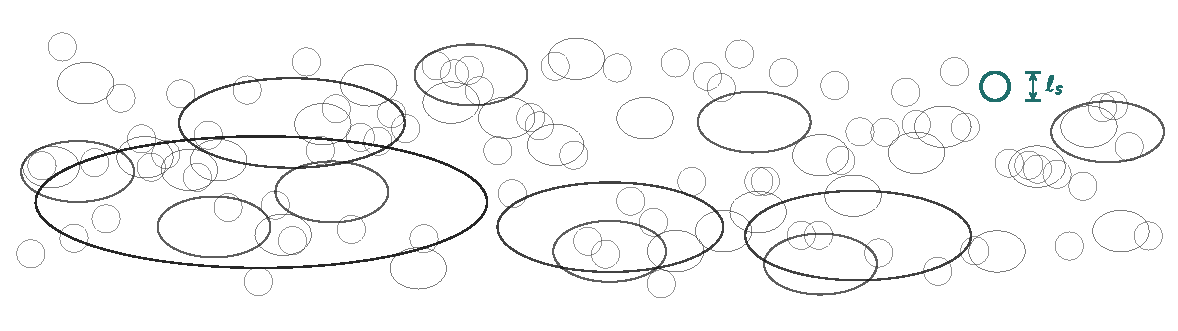
\includegraphics[width=12cm]{concept-figs/v10c_cascade_xz.pdf}
\caption{Vertical slice along an ($x$--$z$) plane of an anisotropic cascade. Ellipses represent the support of individual turbulons of varying size $\ell$ and location. Turbulon aspect ratios follow Eqn. \ref{eq:turbulon aspect ratio scaling} such that large turbulons are horizontally elongated whereas turbulons near in size to the spheroscale $\ell_s$ have unit aspect ratio. Number density per size class is proportional to $\ell^{-(1+H_z)}$, ensuring turbulons of every size class cover the domain.} \label{fig:cascade slice}
\end{figure*}

For simulations, both the shape and relative amplitude at each scale of the turbulons is set by the horizontal hurst exponent $H_h$, the anisotropy exponent $H_z$, and the spheroscale. The canonical values for Lovejoy-Schertzer turbulence are $H_h=1/3$ and $H_z=5/9$ (Eqn. ()), while the spheroscale must be determined empirically. Different values of $H_h$ and $H_z$ can also be used to simulate different turbulent flows, for example isotropic turbulence where $H_h=1/3, H_z=1$. Empirically, values for $H_h$ and $H_v$ are sometimes slightly larger than the canonical Lovejoy-Schertzer values \citet{lovejoy2007,pinel2012,dewitt2025preprint}, while the anisotropy exponent is often closer to its canoical value. For the simulations here, we use $H_h = 0.45$ as found for the wind field by \citet{dewitt2025preprint} and the canonical value $H_z=5/9$. 

One remaining ingredient that is needed for simulations is to determine the constant of proportionality in Eqn. \ref{eq:turbulon amplitude vs scale}. This will set the global mean turbulon amplitude at each scale, and then the final piece will be to specify exactly how amplitudes are distributed spatially, which we consider below. 

At its core, the basic action of a turbulent cascade is to transfer variability from large scales to small scales. In such a downscale cascade, the overall magnitude of the fluctuations at each scale are determined by the amplitude of the fluctuations at the largest scales. For STEAM, this idea is operationalized by computing the large scale fluctuation magnitudes using the ensemble mean profile. For simplicity, we consider a horizontally uniform domain mean, and so the large scale fluctuation magnitude is determined from the ensemble mean profile using differences at the scale of the largest simulated turbulon,  as described in Appendix \ref{sect:steam algorithm details}. This is done individually for each simulated scalar field. The resulting amplitudes at each height are interpreted as the mean absolute amplitude of the turbulon components at the outer scale. 

Using Eqn. \ref{eq:turbulon amplitude vs scale}, outer-scale amplitudes are used to set the proportionality constants for the mean turbulon amplitudes at every other scale. Because the gradient of the mean profile typically varies with height, the proportionality constants will also vary with height. This has two consequences. First, fields which have horizontally and vertically uniform mean profiles will not produce any variability in the simulated scalars, as should be expected. Convective activity should not be expected to modify local concentrations of an already well-mixed gas like argon. Second, any level within the domain that has a stronger mean gradient will produce more small-scale variance, as might also be expected intuitively. Stratocumulus fields near a strong inversion, for example, display much greater moisture variance within in the cloud layer than in the mixed layer below because the proximity to the strong inversion allows for very dry pockets of air to intrude from the free troposphere above. However, as we argue in Sect. (REF), it may be simplistic to set the constant for Eqn. \ref{eq:turbulon amplitude vs scale} using only the gradient magnitude as done here. In the future the sign of the gradient could also be considered.
 
\subsection{Distribution of turbulon amplitudes in space} \label{sect:distribution of turbulon amplitudes in space}

Although Eqn. \ref{eq:LS scalar directional structure functions} constrains the mean absolute turbulon amplitude as a function of scale $\ell$ globally, at any given location a turbulon amplitude should also depend on the local structure of the field. There are two particular aspects to consider: the amount of structure in the scalar field that is available to be advected, and the strength of the eddies that cause such advection to occur. Because advection represents a rearrangement of the field, there must be some nonzero gradient spanning the region in which a given eddy operates if that eddy is to introduce any perturbation in a scalar field. If the scalar field was initially uniform, an eddy might transport molecules from one location to another, but the scalar concentration would not change. If the scalar field does have a nonzero gradient, then it might be expected that the size of the perturbation caused by the eddy would be proportional to the magnitude of the gradient. 

As a first approximation, consider a rearrangement of a linearized gradient in some scalar field $\Phi$. The amplitude of the perturbation due to the rearrangement will be proportional to the gradient magnitude and the length of the eddy that causes this rearrangement. Since the eddies are highly aniostropic, they have very different vertical and horizontal lengths, so we can model advection by introducing a perturbation that is proportional to 
\begin{align}
  \delta \Phi \propto \ell\left|\nabla_h \Phi\right| + \ell_z\left|\frac{\partial \Phi}{\partial z}\right|, \label{eq:anisotropic gradient weighing}
\end{align}
where $\nabla_h$ represents the horizontal component of the gradient operator.

The second aspect of local field structure to consider is the strength of the eddy that causes a perturbation. In a turbulent cascade, eddy strength is determined by the down-cascade turbulent flux, i.e. the dynamically-relevant quantity that is conserved as it is passed from large scales to small. In isotropic Kolmogorov turbulence this quantity is the kinetic energy dissipation rate $\varepsilon$. In Lovejoy-Schertzer turbulence, there are two such fluxes $\varepsilon_h$ and $\phi$ (Eqn. \ref{eq:LS directional structure functions}), with the relevant flux dependent on the direction of the flow. To model eddy strength, STEAM simulations include a normalized flux quantity $\mathcal{F}$ as a prognostic variable alongside $h$ and $q_t$. The main difference between the turbulent flux and the scalar fields is that the turbulent flux is conserved at each scale through the cascade, implying that the amplitude of the flux component of the turbulons does not depend on scale, at least on average. Instead, at each scale $\ell$ the mean absolute perturbation $\langle |\mathcal{F}_\ell |\rangle$ is equal to a constant that is independent of $\ell$, specified by the value of the nondimensional parameter $c_\mathcal{F}$. Because we use a normalized and dimensionless quantity for $\mathcal{F}$, the exact physical nature of the flux is not important and might depend on the flow being simulated. The important property for a turbulent flux is that it is conserved across scale. For each turbulon, we assume that the magnitude of the conserved scalar field component is proportional to the amplitude of the flux component.

The flux $\mathcal{F}$ is not spatially uniform. Local regions within a convective cell will have higher eddy dissipation rates than adjacent clear air, for example. We hypothesize that perturbations in the flux field at scale $\ell$ form with a mean absolute amplitude that is proportional to the local value of $\mathcal{F}_{>\ell}$, that is, the flux field associated with turbulons larger than scale $\ell$. As show in Appendix (), this hypothesis naturally creates multiplicative intermittency in the flux field $\mathcal{F}$, with the strength of the intermittency determined by the mean absolute fluctuation perturbation $\langle |\mathcal{F}_\ell |\rangle$, or equivalently $c_\mathcal{F}$.

Thus, the flux controls the strength of the eddies while the scalar gradient controls the concentration that is available to be advected. Together, in STEAM these physical effects are modeled as follows, described in further detail in Appendix (). The simulation proceeds from large scales to small. At each scale, the first step is to compute perturbations in $\mathcal{F}_\ell$ that are associated with each turbulon of size $\ell$. This is done by drawing a random variable with zero mean and unit amplitude from the distribution described in Appendix (), and then scaling the perturbation by the local field $\mathcal{F}_{>\ell}$ while enforcing that $\langle | \mathcal{F}_\ell | \rangle$ is a constant, independent of scale, with its value determined by the input parameter $c_\mathcal{F}$. Perturbations in $h_\ell$ and $q_{t,\ell}$ are then computed such that the local value is proportional to, from Eqns. \ref{eq:anisotropic gradient weighing} and \ref{eq:turbulon aspect ratio scaling},
\begin{align}
  \delta h \propto \mathcal{F}_\ell\left(\ell|\nabla_h h| + \ell_s^{1-H_z}\ell^{H_z}|\frac{\partial h}{\partial z}|\right) \\
  \delta q_t \propto \mathcal{F}_\ell\left(\ell|\nabla_h q_t| + \ell_s^{1-H_z}\ell^{H_z}|\frac{\partial q_t}{\partial z}|\right).
\end{align}
The proportionality constant is set by enfocing that the ensemble mean $\langle |h_\ell|\rangle$ or $\langle |q_{t,\ell}|\rangle$ follows Eqn. \ref{eq:turbulon amplitude vs scale}. Finally, for all three fields, a perturbation with shape defined by the turbulon envelope function and amplitude scaled as described above are added to the parent fields, and the simulation proceeds to the next smaller scale.

\subsection{Diagnostic variables}

Once the cascade simulation has proceeded to the smallest resolvable scale for the three prognostic variables $h$, $q_t$, and $\mathcal{F}$, we then diagnose additional cloud-relevant variables as described in Appendix (). In short, we use a saturation adjustment scheme where any saturated grid cell is assigned a relative humidity of exactly 100\%, and the remaining water is converted to condensate. Temperatures and pressures that are required for saturation calculations are solved iteratively from the definition of moist static energy, a saturation vapor pressure parameterization (cite bolton1980), and an assumed surface pressure. Condensate is then partioned into liquid and ice according to a simplistic linear partitioning based on the temperature, ramping from purely liquid at 0°C to purely ice at -38°C, matching the partitioning used in the GATE SAM simulation described below. Overall, the diagnostics we use are simplistic and are intended only as a first proof-of-concept that the cascade simulation method can produce plausible simulated atmospheric volumes. A particularly egregious simplification is that condensate does not convert to precipitation, which can lead to unphysically high condensate values in dense convective cores (Sect. (REF PDF SECT)). In the future, precipitation could be added through an autoconversion process analogous to LES, where larger, saturated turbulons produce precipitation over their lifetime. Additional microphysical processes, perhaps including aerosol-limited condensation that produces positive supersaturation, should also be added.



\section{Evaluation of STEAM simulation output}

As a comparison for STEAM outputs, we consider output from two complementary sets of hydrodynamic simulations as well as satellite imagery derived from MODIS. The primary hydrodynamic comparison is to observationally constrained large-eddy simulations of deep convection, referred to as ``giga-LES'' simulations because their numerical grids contain over a billion points. The second hyrdodynamic comparison is to a multimodel ensemble of coarser cloud-resolving simulations from the Radiative-Convective Equilibrium Model Intercomparison Project \citep[RCEMIP;][]{wing2018, wing2020}. Using STEAM and the giga-LES simulations, we also construct simulated cloud masks that are analogous to satellite imagery and compare their statistics to real MODIS imagery.

\subsection{Hydrodynamic comparisons and configuration of STEAM simulations}

The two giga-LES cases were performed with the System for Atmospheric Modeling \citep[SAM;][]{khairoutdinov2003} with identical grid configurations spanning $204.8\,\unit{km}\times204.8\,\unit{km}$, using a doubly periodic domain with $100\,\unit{m}$ horizontal grid spacing and a vertical grid spacing of $100\,\unit{m}$ through the mid-troposphere.
For the first case, boundary conditions were taken from conditions observed during the Tropical Warm Pool -- International Cloud Experiment (TWP-ICE), which sampled monsoonal deep convection near Darwin, Australia in early 2006. The simulation was forced by large-scale thermodynamic tendencies derived from the observed conditions, following the specifications of the TWP-ICE cloud-resolving model intercomparison \citep{dazlichGigaLarge2013, fridlind2010}.
Because only two hours of giga-LES output were preserved, we use a single snapshot taken from the statistically steady portion of the simulation. Th simulated wind field for this case was previously shown to closely follow the directional structure function predictions of Lovejoy-Schertzer turbulence (Eqn. \ref{eq:LS directional structure functions}) \citep{dewitt2025bpreprint}.

The second giga-LES case is forced by idealized mean conditions observed during Phase III of the Global Atmospheric Research Program Atlantic Tropical Experiment (GATE), which sampled oceanic deep convection over the tropical east Atlantic in 1974 \citep{khairoutdinov2009}. In contrast to the time-varying TWP-ICE forcing, the prescribed large-scale tendencies are constant in time. Over the 24-hour simulation, convection develops from shallow cumulus into deep convection within the first six hours and is quasi-steady beyond approximately hour 12 \citep{khairoutdinov2009}. We use a single snapshot taken from hour 23.
% CLAUDE: verify the GATE snapshot choice -- dewitt2024 analyzed hourly output over hours 12-24; adjust "final hour" if a different snapshot (or several) is used here.

Both giga-LES simulations are constrained by observations. Large-scale advective tendencies of temperature and moisture are prescribed as horizontally uniform profiles, and the horizontal mean wind profile is relaxed toward the observed mean profile \citep{khairoutdinov2009, fridlind2010}. The TWP-ICE case additionally has its horizontal mean temperature and humidity profiles relaxed toward observed profiles above ${\sim}15\,\unit{km}$, where the observationally derived forcing tendencies are poorly constrained \citep{fridlind2010}. STEAM's use of specified mean profiles for $h$ and $q_t$ is a stronger constraint than the tendencies prescribed in SAM, but it is analogous in the sense that only the horizontal mean is prescribed. In both the giga-LES and in STEAM, all local variability arises from the intrinsic dynamics of the model.

The RCEMIP ensemble provides a complementary form of evaluation. RCEMIP simulations are run in radiative-convective equilibrium, an idealization of the tropical atmosphere in which convection interacts with interactive radiation and surface fluxes over a fixed, horizontally uniform sea surface temperature, with spatially uniform insolation, no rotation, and no diurnal cycle \citep{wing2018}. Radiative-convective equilibrium is a less realistic boundary condition than the forcings prescribed for the giga-LES simulation. It is included here as a complementary evaluation that establishes the magnitude of the variability present between different hydrodynamic models even under identical forcings. 

We use the \texttt{RCE\_large300} configuration: an elongated, doubly periodic channel of approximately $6000\times400\,\unit{km}^2$ with $3\,\unit{km}$ horizontal grid spacing and a sea surface temperature of 300 K, integrated for 100 days. In this configuration, convection produces moist convecting regions and dry, nearly cloud-free regions whose number, spatial scale, and orientation differ among models \citep{wing2020}. 

From the RCEMIP archive we use the nine models hat provide usable three-dimensional snapshot output for the 300 K channel: SAM, CM1, SCALE, UCLA-CRM, three configurations of the Met Office Unified Model, and two configurations of ICON. We use three snapshots separated by ten days near the end of the integration, chosen so that each snapshot is equilibrated and approximately statistically independent. Two archived models are excluded for data integrity reasons. A complete specification of the comparison data and analysis is provided in the supplement.
Notably, SAM appears in both comparison sets, at $100\,\unit{m}$ resolution for the giga-LES cases and at $3\,\unit{km}$ resolution in RCEMIP. The hydrodynamic ensemble therefore contains a shared underlying model spanning very different domain and boundary condition configurations (SAM), while also containing a set of shared domain and boundary condition configurations that span very different underlying models (RCEMIP).

In any hydrodynamic simulation, statistics computed at the grid scale are often strongly affected by numerical approximations such as hyperdiffusion or filtering that tend to damp grid-scale variability. A model's ``effective'' resolution is often considered to be a few times larger than the grid spacing due to these approximations (citation). As we will show, our findings using fluctuation functions, which measure variability across different scales, corroborate the idea that a model's effective resolution is larger than its grid spacing. In contrast, STEAM's effective resolution is equal to the grid spacing because it does not contain the same approximations.

A distinct but closely related challenge is that simple statistics such as standard deviation depend strongly on the resolution used to compute them, especially for scale invariant fields \citep{lovejoy2013}. To account for both of these methodological subtleties, for all one-point statistics such as standard deviations, we first coarsen hydrodynamic outputs in $2\times 2\times 2$ blocks to reduce numerical artifacts, and then configure STEAM comparisons such that both horizontal and vertical resolutions are nearly matched between STEAM and the hydrodynamic comparison (see Supplement). Analysis functions that measure variability across scales, such as fluctuation functions and cloud fractal metrics, are computed at native resolution in order to show numerical artifacts directly.

In order to match resolutions, and because STEAM requires parameters such as mean profiles to be specified as inputs, we construct matching STEAM configurations for each individual hydrodynamic case. We refer to a given configuration of the hyrdodynamic model as the ``host'' model. Most importantly, the mean vertical profiles of the prognostic variables $q_t$ and $h$ are required as inputs to STEAM, and these are computed from the host model output. STEAM also requires a profile for the spheroscale, a constant $c$ specifying the amount of intermittency in the flux, and a constant for the outer scale. 

The outer scale $L$, which represents the size of the largest turbulon, is most simple. It is set to the domain length, so that the largest turbulon is defined to be simply the largest that could fit inside the domain. For the channel configurations, it is ambiguous which domain length constrains the size of the largest turbulon, so we consider two comparisons for the channel cases: the outer scale being set to either the channel width or length. For the spheroscale profile, we use a uniform value of $10\,\unit{m}$ which is consistent with observations \citep{dewitt2025preprint}. As we discuss in Section (), in the real atmosphere the spheroscale is likely to display large spatial variability, so the constant used here is a key approximation that we return to in Sect. (REF VISUALIZATION SECTION) It is less clear what the value for the flux perturbation scaling factor $c$ should be, and it is more difficult to constrain observationally. We consider three cases: $c\in{0.02,0.05, 0.17}$.



\subsection{Comparison between hydrodynamic- and STEAM-simulated fields}

We begin our comparison using profile statistics and per-level PDFs for fields simulated by STEAM and the hydrodynamic models. These comparisons are made between coarsened hydrodynamic models and STEAM simulations with domain geometry and mean profiles for $h$ and $q_t$ matched to each hydrodynamic case.


STEAM shows some agreement with several notable departures from the host models. In both GATE and TWPICE, the upper-level peak in cloud fraction occurs at nearly the same altitude as it does in the host simulation, but the magnitude only matches for the GATE case, and in all cases STEAM produces roughly 2-5x higher cloud fraction at lower levels. Standard deviations for liquid and ice condensate are generally higher in STEAM, with the exception of the GATE case where STEAM standard deviation for $q_i$ is more comparable to its host. For variability in $h$, STEAM agrees relatively well with its host below approximately 12~km and reproduces the low-level peak. At upper levels STEAM has far higher variability in $h$, which also drives a peak in temperature variability there. At lower levels, STEAM also has 2-4$\times$ more variability than either hydrodynamic simulation, but at least some snapshots are closer to their hydrodynamic hosts in the mid troposphere between about 5~km and 12~km.

The high altitude peak in $h$ and $T$ variability, along with higher variability in $q_c$ and, to a lesser extent higher low-level cloud fraction, are the clearest departures between STEAM and the host simulations. A less obvious departure is $h$ and $q_t$ variability at the surface, where variability drops in all models but only reaches zero in STEAM. Elsewhere, departures between STEAM and the host model are generally of a comparable magnitude to departures between the two hydrodynamic models themselves. Intruigingly, the value of the flux perturbation scaling parameter $c$ appears not to substantially affect profiles for standard deviation, full plots for which are shown in Appendix ().

\begin{figure}
  \caption{
Standard deviation profiles of moist static energy $h$, total water mixing ratio $q_t$, cloud liquid and ice mixing ratios $q_c$ and $q_i$, temperature $T$, and cloud fraction. For STEAM, profiles (yellow lines) are computed from five statistically independent fields for the moderate value $c_\mathcal{F}$, using the TWPICE or GATE profiles for $h$ and $q_t$ as inputs. Profiles for other values of $c_\mathcal{F}$ are shown in Appendix () and not substantially different from the $c_\mathcal{F}=0.05$ case. Standard deviation profiles for the hydrodynamic simulations (black lines) are instead computed using only a single statistically independent snapshot. The grey shading represents snapshot-to-snapshot variability in STEAM, showing the minimum and maximum at every height for profiles computed for each individual STEAM field, spanning the five ensemble members and three values for $c_\mathcal{F}$.}
\end{figure}

The probability density functions for 5~km and 10~km altitudes shown in Fig. () show general agreement between the host and STEAM outputs, and in this case the effect of changing $c$ is more noticable. In nearly all cases the host PDF is bracked by the STEAM outputs across values for $c$, with larger values for $c$ showing fatter tails in the distributions.

Similar trends are present in the RCEMIP comparison, at least for the configuration where the outer scale is set to the channel width (Fig. ()).  For these cases, at least some STEAM profiles are overlapping with at least some RCEMIP profiles for most variables and heights. The most notable exception is again high-elevation moist static energy and temperature variability, which is substantially higher for STEAM. Surface-level variability in $h$ and $q_t$ is also lower for STEAM. For liquid condensate, most STEAM members show vastly higher variability, although the dryest STEAM members overlap the wettest RCEMIP members at all levels. For ice condensate, the STEAM and RCEMIP ensembles are very similar. Profiles for the alternate configuration with larger outer scale are shown in Appendix (), where variability is generally increased.

Increased variability of liquid condensate in STEAM would be consistent with values for $q_c$ being artificially inflated in because precipitation is not present in the model. The high-altitude peak in $h$ and $T$ variability likely arises because the mean profile for $h$ warms sharply at the tropopause, where STEAM's gradient weighting mechanism (Eqns. REF) reads a substantial large-scale gradient and cascades that large-scale variability down to smaller scales. In the real atmosphere, the stratospheric inversion instead suppresses motion, suggesting that in the future, not only the magnitude of the large scale vertical gradient, but also the sign, should matter for STEAM's dynamics. Both aspects suggest future work is needed to address these limitations in STEAM. 

The broad agreement elsewhere is promising and, in some sense, somewhat remarkable. In these simulations, STEAM reads only the large-scale vertical gradient in the mean profile, translates this into a horizontal perturbation, and then extrapolates that perturbation over approximately a factor of 1000 in horizontal scale. That the resulting variability at each horizontal level would match that of a hydrodynamic model even to within an order of magnitude is not obvious a priori.


Moving beyond one-point statistics, we now consider fluctuation functions as defined in Equation \ref{eq:wavelet transform}, computed for 5~km and 10~km levels in the horizontal direction using a Mexican Hat wavelet. Computations are performed using the Python package \verb|scaleinvariance| (CITATION). To estimate power-law exponents, we use a linear regression to the logarithm of the fluctuation function vs. the logarithm of the scale parameter. To better examine the scaling behavior, we define a ``local exponent'' for each scale $r$, which represents the power-law exponent fit to scales within the half order-of-magnitude surrounding $r$. This function is plotted in Fig. () next to the fluctuation functions themselves for moist static energy $h$ and total water content $q_t$ for the giga-LES comparison. For a scale-invariant power-law function with a constant exponent, the local exponent will be constant with scale, as it is for STEAM and the TWPICE SAM case at mid-range scales near 10~km. As the scale is increased toward the outer scale, in all cases the flutuation function rolls off and local slopes decrease toward zero. The outer scale is plausibly 2 to 4 times smaller in the TWPICE hydrodynamic simulation than in STEAM. Local slope plots for the SAM GATE simulation are much less constant, indicating that simulation is substantially less scale invariant than either STEAM or the other hydrodynamic case. Also notable is that the magnitude of the fluctuation functions agrees with the TWPICE case over much of the observed range, while for GATE fluctuation function magnitudes are much lower, particularly for the 10~km altitude slice.



\subsection{Comparison of simulated and observationally-derived satellite imagery}

A complementary way of evaluating STEAM simulation output is to consider the geometry of cloud objects as if they were viewed from space. Because atmospheric clouds are fractal, it is most natural to quantify their geometry by considering scale invariant metrics \citep{dewitt2026}. Such metrics are also well suited for comparisons between models and observations with differing resolutions, such as the giga-LES and satellite observations we consider here. This is because they represent statistical relationships across many different scales rather than at any single scale, and so their value is not affected by resolution unlike the metrics considered in Sect. (PREVIOUS SEC) \citep{dewitt2026}. 

Most generally, such metrics quantify how some measure of cloud structure scales with some measure of cloud size. We consider four specific metrics relating cloud structure to cloud size that are defined below: the individual and ensemble fractal dimensions $D_f$ and $D_e$ and size distribution exponents for cloud area $\tau_\mathrm{area}$ and perimeter $\tau_{\mathrm{per.}}$. 
The first metric, the individual fractal dimension, measures how convoluted individual cloud perimeters become as the cloud under consideration grows larger. It is defined by measuring the rate at which individual cloud perimeters increase as the cloud's bounding box area grows, with higher values indicating a more convoluted perimeter. 
The second dimension is the ``ensemble'' fractal dimension, which quantifies both how convoluted individual cloud perimeters are in addition to the relative frequency of small and large clouds. The dimension is obtained via a linear regression to a logarithmically-transformed plot of the count of cloud-edge pixels that are separated less than a distance $r$, a function known as the ``correlation integral''.  The computation of both fractal dimensions follows the recommendations of \citet{dewitt2026}.
The third and fourth metrics, the size distribution exponents $\tau_\mathrm{area}$ and $\tau_{\mathrm{per.}}$, are computed using a linear regression to a logarithmically-transformed histogram of cloud area or perimeter. 

An extensive theoretical, empirical, and methodological investigation of all four metrics was described in \citet{dewitt2024,dewitt2024b} and \citet{dewitt2026}, with recommendations implemented in the Python package \verb|objscale|. We defer further methodological details and choices to those papers and use \verb|objscale| functions with defaults for the computation of the four metrics.

Accurate calculation of these metrics requires resolving a wider range of cloud sizes than are present in the narrow RCEMIP channels \citep{dewitt2024b}, and single snapshots the giga-LES cases provide are only statistically robust for the fractal dimensions. We therefore exclude RCEMIP entirely and only report $D_e$ and $D_f$ for the giga-LES cases.

As an additional point of comparison, we compute the fractal metrics for a selection of 72 satellite images, collected using MODIS between January 1-10. These particular granules were filtered by \citet{dewitt2026} to remove granules containing sun glint and are entirely over ocean, so that a simple reflectivity-based threshold may be used to define cloud boundaries. 

STEAM simulations are constructed with a domain geometry that is broadly similar to MODIS, using a $1\,\unit{km}$ horizontal grid spacing in a square domain spanning $2048\times 2048\,\unit{km}$. Both are comparable to the resolution and extent of the MODIS imagery, which has a nadir resolution of approximately $1\,\unit{km}$ and a domain size of (FILL THIS IN). For each value of the flux perturbation magnitude $c$, we simulate ten independent STEAM volumes.

For both STEAM and the giga-LES volumes, simulated albedo fields are constructed by first computing a column optical depth field $\tau_c$ from the liquid and ice water paths, as implemented in the \verb|cloudyview| Python package as
\begin{align}
  \tau_c = \frac{3}{2}\frac{\mathrm{LWP}}{\rho_w\, r_{e,\mathrm{liq}}} + \mathrm{IWP}\left(a + \frac{b}{r_{e,\mathrm{ice}}}\right), \label{eq:bulk optics}
\end{align}
where the liquid and ice water paths $\mathrm{LWP}$ and $\mathrm{IWP}$ are obtained by vertically integrating the condensate fields within each column, $\rho_w$ is the density of liquid water, and the assumed effective radii are $r_{e,\mathrm{liq}} = 10\,\unit{\mu m}$ and $r_{e,\mathrm{ice}} = 30\,\unit{\mu m}$. The liquid term is the geometric optics relationship from \citet[Eq. 7.86 of][]{petty2006} and the ice term is the visible-band ice parameterization of \citet{ebert1992}, with $a = 3.448\times10^{-3}\,\unit{m^2\,g^{-1}}$ and $b = 2.431\,\unit{\mu m\, m^2\,g^{-1}}$ for water paths in $\unit{g\,m^{-2}}$. 

From the column optical depth, visual albedo is computed using the two-stream solution for the reflectivity of a nonabsorbing cloud layer \citep[Eq. 5.51 of][]{bohren2006}:
\begin{align}
  A = \frac{(1-g)\,\tau_c}{(1-g)\,\tau_c + 2}, \label{eq:two stream albedo}
\end{align}
with asymmetry parameter $g = 0.85$. With the solar zenith adjustment described in the supplement, MODIS reflectivity and model albedo are comparable for clouds. For both, cloud masks are defined by thresholding the albedo or reflectivity using thresholds of $R \in \{0.1, 0.2, 0.3\}$. Because $A$ increases monotonically with $\tau_c$, each albedo threshold is equivalent to a threshold in column optical depth, with the three values of $R$ corresponding to $\tau_c \approx 1.5$, $3.3$, and $5.7$.

With the possible exception of the TWPICE giga-LES case at R=0.3, all of the geometric scaling functions are well represented by a power law, with a local scaling exponent differing by no more than (VALUE) across the measured scaling range as shown in Appendix (). 

\begin{table*}[t]
\caption{Cloud geometric exponents as a function of reflectance threshold $R$ for STEAM, the giga-LES hydrodynamic model SAM, and MODIS observations. $D_e$ is the ensemble fractal dimension, $D_i$ the individual fractal dimension ($D_i$ in DeWitt et al., 2026), and $\tau_{\mathrm{area}}$, $\tau_{\mathrm{per}}$ the size distribution exponents for individual cloud area and perimeter. ``CF'' is cloud fraction. Bolded model-derived estimates represent those that are closest to the MODIS value. Estimates are not reported when they fail the statistical robustness checks described in the Supplement as recommended by \citet{dewitt2024b, dewitt2026,dewitt2025objscale}.}
\label{tab:cloud geometry}
\begin{tabular}{lccccc}
\tophline
 & CF & $D_e$ & $D_f$ & $\tau_{\mathrm{area}}$ & $\tau_{\mathrm{per}}$ \\
\middlehline
\multicolumn{6}{l}{\textbf{$R > 0.1$}} \\
MODIS & 0.54 & 1.77 & 1.37 & 0.85 & 1.27 \\
\cline{1-6}
SAM-GATE & 0.31 & 1.68 & 1.50 & \textit{1.14} & \textit{1.53} \\
SAM-TWPICE & 0.95 & 1.47 & -- & \textit{0.38} & \textit{0.97} \\
STEAM $c = 0.02$ & 0.51 & 1.60 & 1.27 & 0.67 & \textit{1.10} \\
STEAM $c = 0.05$ & 0.51 & 1.64 & \textbf{1.30} & 0.71 & 1.14 \\
STEAM $c = 0.17$ & \textbf{0.53} & \textbf{1.74} & \textbf{1.31} & \textbf{0.81} & \textbf{1.23} \\
\middlehline
\multicolumn{6}{l}{\textbf{$R > 0.2$}} \\
MODIS & 0.41 & 1.75 & 1.40 & 0.88 & 1.28 \\
\cline{1-6}
SAM-GATE & 0.23 & 1.62 & \textbf{1.28} & \textit{1.02} & \textit{1.40} \\
SAM-TWPICE & 0.78 & 1.57 & 1.19 & \textit{0.58} & \textit{1.12} \\
STEAM $c = 0.02$ & \textbf{0.47} & 1.60 & 1.27 & 0.66 & 1.04 \\
STEAM $c = 0.05$ & \textbf{0.48} & 1.63 & 1.27 & 0.71 & 1.10 \\
STEAM $c = 0.17$ & 0.49 & \textbf{1.73} & \textbf{1.29} & \textbf{0.80} & \textbf{1.22} \\
\middlehline
\multicolumn{6}{l}{\textbf{$R > 0.3$}} \\
MODIS & 0.32 & 1.73 & 1.38 & 0.89 & 1.29 \\
\cline{1-6}
SAM-GATE & \textbf{0.19} & 1.58 & 1.24 & \textbf{\textit{0.96}} & \textit{1.40} \\
SAM-TWPICE & 0.58 & 1.61 & 1.21 & \textit{0.62} & \textit{1.13} \\
STEAM $c = 0.02$ & \textbf{0.44} & 1.58 & 1.24 & 0.64 & 1.02 \\
STEAM $c = 0.05$ & \textbf{0.45} & 1.62 & 1.26 & 0.70 & 1.07 \\
STEAM $c = 0.17$ & 0.46 & \textbf{1.72} & \textbf{1.28} & 0.79 & \textbf{1.20} \\
\bottomhline
\end{tabular}
\belowtable{}
\end{table*}

The calculated values of the geometric exponents are shown in Table \ref{tab:cloud geometry}. The only parameter that can be reliably estimated in all datasets is the ensemble fractal dimension $D_e$, for which the highly intermittent STEAM case agrees best with MODIS across all thresholds defining cloud. The hydrodynamic model reproduces the individual fractal dimension better than the STEAM for two out of three thresholds. Measured size distribution exponents for the STEAM highly intermittent case generally agree with MODIS estimates to within $0.15$, which is comparable to the deviation in power-law behavior in MODIS as shown in Appendix ().  However,  the single hydrodynamic case for which distribution exponents could be measured (SAM-GATE at $R=0.3$) indicates a value that is closer to MODIS than STEAM. Overall, for all exponent and threshold combinations where there is at least one hydrodynamic and one STEAM exponent, STEAM beats the hydrodynamic models in 4 out of 8 cases, and the more highly intermittent case is substantially closer to MODIS compared to the less intermittent case.

\subsection{Visual renderings of STEAM clouds}

As a final analysis of STEAM outputs, we turn to renderings of simulated clouds. \citet{palmer2016} proposed a ``Palmer-Turing test''\footnote{Referred to there as a ``climatic Turing test''; we use the terminology put forward by \citet{christensen2021}.} as a standard for model fidelity: if simulated output cannot be visually distinguished from observations of the real atmosphere, then for all practical purposes there is no difference between them. Visual realism is of course a bounded form of evidence, but it can be meaningful when paired with quantitative statistics, allowing one to build intuition about what is done well and what is not. As we will show, renderings of STEAM suggest concrete future research directions, and for that alone the exercise is quite valuable.

We use the cloud visualization engine \verb|cloudyview| (CITATION). Because \verb|cloudyview|'s physically-based Monte Carlo engine is computationally intractable for even moderately thick clouds, we use a ray-marching algorithm that uses tuned heuristics for pixel lighting but physically accurate viewing geometry. The algorithm is computationally inexpensive enough that a consumer GPU can render views in real time, as if in a video game. An interactive demo of STEAM-simulated clouds, alongside hydrodynamic comparisons, is available for this purpose at (URL).

We focus here on renderings for a small-domain periodic channel simulation spanning 40.96~km in the longer dimension, 10.24~km in the shorter, and 5.5~km in the vertical. The horizontal grid spacing is set to 20~m for a grid size in the horizontal of 2048$\times$512. Inside this ``parent'' simulation, we also simulated a ``nested'' domain, which is produced by continuing the cascade over a small sub-region of the parent, as described in Appendix \ref{sect:steam algorithm details}. Specifically, within a X by X region of the parent, the cascade is continued to a final horizontal grid spacing of X, cooresponding to a grid size of X by X for the nested domain. Profiles for $h$ and $q_t$ are used from the CM1 channel simulation, which were found to result in cloud fractions that are conducive to visualization. The same nesting procedure can also be performed for the larger domains investigated above to produce renderings, which are shown in Appendix (). 

The first worthwhile visual comparison is between cases with higher and lower intermittency, controlled by the flux perturbation scaling parameter $c$. In Fig. (), a composite image is shown for two small-domain simulations with the same random seed but different values of $c$, so that exactly the same cloud is simulated in both cases but with varying degrees of intermittency. The lower value $c=0.02$ has a smaller cloud fraction in the rendered region and is dominated by larger clouds, as is consistent with the smaller size distribution exponents obtained for this value (Table \ref{tab:cloud geometry}). The higher value $c=0.17$ fills clear regions with more small and dense clouds. 
% This result is in some tension with the finding that the $c=0.17$ case produces the closest match to MODIS observations in Table ().

The other particularly useful visual comparison is the effect of changing the spheroscale. For simplicity, we only used a single constant value of $\ell_s=10\,\unit{m}$ in the quantitative comparison above, given that this parameter has at least been estimated in past work \citep{dewitt2025preprint}, unlike $c$. Nonetheless, a constant value is unlikely to be realistic. Consider the renderings shown in Fig. () for spheroscales 10~m, 30~m, and 100~m. Each case is visually realistic but displays a different type of cloud: smaller values create thin, scattered cumulus, while larger spheroscales cause cumulus congestus to form. It seems likely that spheroscales in deep convection grow much larger still, perhaps to a few kilometers or even more (CITE LOVEJOY APPX REVIEW). 

All simulations here have a spheroscale that is prescribed to be a constant, so that deep convective cores are exactly as stratified as thin, scattered cumulus in another part of the domain. In the real atmosphere, clouds with varying spheroscales can clearly coexist. For example, stratified cloud decks are commonly found adjacent to deep convective cores where updrafts reach their level of neutral buoyancy and spread out laterally. A clear future direction for STEAM, then, is to investigate methods to incorporate the spheroscale into the dynamics of the model rather than being prescribed. Concievably, its value should depend on the local stratification in some way: locally unstable regions create more convective clouds while more stable regions create stratocumulus.

The figure displayed in the introduction (Fig. ()) was rendered for a simulation using the small domain configuration. Out of the parameter set visualized here, the values $c=0.02$ and $\ell_s=30\,\unit{m}$ were found to provide the best match to the photograph taken in the summer from Utah's Wasatch mountains. At least for this meteorological condition, we tentatively suggest that STEAM passes the Palmer-Turing test for visual fidelity. Without labels, it might be quite difficult to identify the real image from the simulated one.


\section{Conclusions}

Even setting aside the challenging question of microphysics, fully resolving the dynamics of moist convection would require a domain spanning hundreds of kilometers but with grid spacings near millimetric scales. Sufficent computers can only be found in science fiction. 
In the real world, we are instead forced to come up with simplified representations of far more numerous and complex small-scale interactions. Such a representation is usually referred to as a parameterization, which almost undersells the problem. What is needed is an emergent theory for atmospheric dynamics, one that arises from, and accounts for, billions of complex small-scale interactions without explicitly simulating them.

Several nascent attempts at such a theory exist, but none are yet developed enough to make plausible simulations of a moist convective atmosphere. 
Here, we develop a generalization of turbulence theory that applies to stratified atmospheres, originally proposed by \citet{schertzer1985}. Our modifications are sufficient to produce numerical simulations of three-dimensional moist thermodynamic quantities that are broadly comparable to existing state-of-the-art hydrodynamic simulations.
The central idea is to formalize and generalize the concept of a ``turbulent eddy'', and to replace it with a mathematical object we term a ``turbulon''. A convective cloud field, then, is nothing more than a superposition of a large number of turbulons. 

Cloud fields simulated with STEAM are plausible but do not match those coming from existing state-of-the-art hydrodynamic models in every way. As we show, some departures are expected a priori, some are unexpected but suggest clear improvements, and some remain mysterious. Even so, STEAM is promising as a method of simulating Earth's atmosphere without using the equations of hydrodynamic motion at all, analogous to how fluid mechanical simulations themselves simulate fluid flow without using the equations of quantum mechanics. The model requires a few physical constants and ensemble-mean profiles for moist static energy and total mixing ratio, and outputs three-dimensional fields for moist static energy, water vapor, cloud liquid and ice condensate, temperature, and pressure. Horizontal and vertical variability of the generated fields is broadly similar to that computed for state-of-the-art hydrodynamic simulations.
Comparing simulated albedo fields from STEAM clouds and hydrodynamic models to MODIS imagery suggests that STEAM clouds are, surprisingly, more aligned with MODIS observations than the hydrodynamic models, raising the possibility that STEAM's discrepancies with the hydrodynamic models could, in some cases, indicate a deficiency in the hydrodynamic model rather than STEAM.

Using a cloud rendering algorithm, we suggest that STEAM tentatively passes the ``climactic Turing test,'' where outputs are visually indistinguishable to the human eye, at least for some cloud types. These visualizations, combined with the quantitative analysis, suggest concrete future research directions, mainly investigating models where the spheroscale varies spatially, investigating the role of the intermittency parameter, and improving STEAM's simplistic treatment of stable profiles found at the tropopause.

Perhaps most surprising is STEAM's computational advantage, estimated rigorously in the Supplement. Primarily because the model is not time dependent and therefore does not require computation of intermediate states, STEAM simulations are $\sim 10^5\times$ faster per independent snapshot than the hydrodynamic model CM1 on the same hardware. If the limitations we discuss can be addressed, perhaps fully resolving a convective system is not science fiction after all. The real question is whether it would be necessary, or if an emergent physical theory for atmospheric dynamics is all that is needed.


\clearpage




























% \conclusions  %% \conclusions[modified heading if necessary]


%% The following commands are for the statements about the availability of data sets and/or software code corresponding to the manuscript.
%% It is strongly recommended to make use of these sections in case data sets and/or software code have been part of your research the article is based on.

% \codeavailability{TEXT} %% use this section when having only software code available


% \dataavailability{TEXT} %% use this section when having only data sets available


% \codedataavailability{TEXT} %% use this section when having data sets and software code available


% \sampleavailability{TEXT} %% use this section when having geoscientific samples available


% \videosupplement{TEXT} %% use this section when having video supplements available


\appendix

% \section{math details}


% \subsection{Turbulon envelope shape}

% Although Eq. () ensures that any admissible envelope function may be used to construct simulations of a turbulent field, not all envelope functions are physically realistic.

% If $\mathfrak{T}$ is chosen so as to have zero mean, the mathematical formalism of wavelet transforms guarantees that it is possible to construct any possible field $F$ using this setup. In fact, wavelet theory supplies a universal method to convert any state of the system between a real-space field description $F(\mathbf{r})$ and a "turbulon space" description, i.e. a description of the system in terms of a list of turbulon amplitudes as a function of location and $k$:
% \begin{align}
%   a(\mathbf{r}, k) &= \int F(\mathbf{r}') \mathfrak{T}^*_k(\mathbf{r} - \mathbf{r}') d^3\mathbf{r}'.
% \end{align}
% As a note, our approach in Eqns. () and () differs slightly from a continuous wavelet transform. When constructing simulations, for computational reasons we only consider a sparse subset of possible turbulon locations where the spacing between allowable locations is proportional to $k$. This affects the wavelet normalization factor and is discussed in detail in Appendix ().
% As for the shape of $\mathfrak{T}$, there are few constraints beyond the requirement of zero mean. As a starting point, we will use the Mexican hat, defined as 
% \begin{align}
%   whatever.
% \end{align}
% The Mexican hat is a common choice in wavelet analysis, and in Sect. () we will explore several alternatives. As a final note, for constructing simulations it is convenient for $\mathfrak{T}$ to also have finite gradient as discussed in Sect. (), but for analysis a finite gradient is not required.


% For our purposes, the structure function is advantageous compared to the kinetic energy spectrum because it does not need to be defined with respect to variance $\Delta v^2$. Structure functions may be defined for any order $q$:
% \begin{align}
%   \langle\Delta v^q (r)\rangle\equiv \langle |v(\mathbf{x})-v(\mathbf{x}+\mathbf{r})|^q\rangle.
% \end{align}
% This generalized definition is useful because if we set $q=1$, the structure function may be recast as a wavelet or a turbulon envelope function:
% \begin{align}
%   \langle\Delta v^2 (r)\rangle = v * \mathfrak{T}; \qquad
%   \mathfrak{T} = -\delta(-\mathbf{r}/2)+\delta(\mathbf{r}/2)
% \end{align}
% where $\delta$ is the Dirac delta function. This implies that we may interpret velocity differences $\Delta v$ as turbulons, and therefore their mean amplitude as a function of scale $k=r$ is constrained via the Hurst exponent in Eqn. \ref{eq:LS directional structure functions}. This illustrates a more general feature of the turbulon representation of a turbulent flow: even if we do not use differences to represent turbulons, their mean amplitude remains constrained by Eqn. \ref{eq:LS directional structure functions}.


\section{STEAM algorithm} \label{sect:steam algorithm details}

Here we provide an explicit description of the STEAM algorithm for modeling moist static energy $h$, total water mixing ratio $q$, and the conserved turbulent flux $\mathcal{F}$.
As a point of notation, there are three distinct types of averages requiring disambiguation. Consider a large ensemble of statistically independent turbulent flows. Any variable may be averaged along the spatial directions, which we denote $\langle \rangle_\mathbf{x}$, or alternatively $\langle \rangle_\mathbf{x}(z)$ when the average is taken over the horizontal dimensions only. The result may in principle still have time dependence and differ between ensemble members. Alternatively, if we average only along the time direction, denoted by $\langle \rangle_t$, in principle the result may differ spatially and among ensemble members. Finally, we might average across ensemble members, which we denote $\langle \rangle_i$, which in principle could result in an ensemble mean that still varies in time and space. When ergodicity applies, such as in an RCE simulation, $\langle \rangle_t=\langle \rangle_i$. Unit vectors are denoted as $\hat{x}, \hat{y}, \hat{z}$, and we denote the horizontal gradient magnitude of some arbitrary field $f$
\begin{align}
  |\nabla_h f| = \sqrt{\left(\frac{\partial f}{\partial x}\right)^2 + \left(\frac{\partial f}{\partial y}\right)^2}.
\end{align}
For an arbitrary variable $\Phi$, we refer to the component of $\Phi$ that is associated with perturbations of a given size class $\ell$ as $\Phi_\ell$. The component of $\Phi$ associated with perturbations of size larger than $\ell$ is written $\Phi_{>\ell}$, so that 
$$\Phi = \langle \Phi \rangle_t + \sum_{\ell'=\ell_\text{min}}^{\ell'=L} \Phi_{\ell'},$$
$$\Phi_{>\ell} = \langle \Phi \rangle_t + \sum_{\ell'>\ell}^{L} \Phi_{\ell'} ,$$
$$\Phi_{\ge\ell} = \langle \Phi \rangle_t + \sum_{\ell'=\ell}^{L} \Phi_{\ell'} .$$

We assume the ensemble means $\langle h \rangle_t$ and $\langle q_t \rangle_t$ are known and horizontally uniform, in which case they may be simply represented by a 1D profile along the vertical direction. We also assume the outer scale $L$ and the spheroscale $\ell_s$ are known, along with physical bounds $[\Phi_{\min}, \Phi_{\max}]$ for each advected scalar, and we consider logarithmically-spaced size classes for the turbulons such as $L, L/2, L/4, \dots, 2dx$, implying the outer scale must be a power of two factor of the horizontal grid resolution. The smallest size class is $2dx$ rather than $dx$ so that the finest turbulons are Nyquist-sampled by the output grid. The cascade density may be increased to an integer $n_c\ge 1$ size classes per octave, so that adjacent classes are separated by the scale ratio $2^{1/n_c}$. When $n_c>1$, an adjustment factor described below is included to compensate for the increased variance due to more size classes. The simulations here use dyadic classes, $n_c = 1$.

First, define the three-dimensional turbulon envelope shape $\mathfrak{T}_\ell$ as a function of size class $\ell$. For simplicity we will use the three-dimensional Mexican hat (the negative Laplacian of a Gaussian) with width parameter $\sigma = \ell/\pi$, chosen so that the envelope's power spectral density peaks near wavelength $\ell$:
\begin{align}
  \mathfrak{T}_\ell(||r||) = \left(\delta -\frac{\pi^2||r||^2}{\ell^2}\right)\exp \left(-\frac{\pi^2||r||^2}{2\ell^2}\right) \label{apxeq:turbulon shape}
\end{align}
Here, $||r||$ is a vertically-stretched distance metric defined by
\begin{align}
  ||r|| = \left(x^{2} +y^{2} + \left(z\frac{\ell}{\ell_z}\right)^{2}\right)^{1/2}. \label{apxeq:stretched distance}
\end{align}
The familiar one-dimensional Mexican hat would have $\delta = 1$, but $\delta$ must be modified in order to keep $\mathfrak{T}_\ell(||r||)$ zero mean, both because the wavelet is three-dimensional and because it is resolved on a coarse grid. We use $\delta=2.9678$, a constant computed numerically for default ``sparsity factors'' defined below.

The turbulon aspect ratio $\ell/\ell_z$ is defined by
\begin{align}
  \begin{cases}
    \ell_z>\ell_s; \qquad \ell_z = \ell_s \left(\frac{\ell}{\ell_s}\right)^{H_z}, \\
    \ell_z \le \ell_s; \qquad \ell_z = \ell,
  \end{cases}
   \label{apxeq:vertical turbulon size class}
\end{align}
which recovers Eqn. \ref{eq:turbulon aspect ratio scaling} at scales larger than $\ell_s$ and is isotropic at smaller scales. This piecewise aspect ratio scaling function was found to produce more visually realistic sub-spheroscale clouds (not shown). However, all simulations that are analyzed quantitatively here are fully within the anisotropic regime due to the small spheroscales considered. The visualizations in Sect. () are the only simulations containing sub-spheroscale turbulons.

In practice the stretched metric is realized by constructing an envelope that is isotropic in grid-index space on a working grid whose vertical spacing is compressed in proportion to $\ell_z/\ell$ (see the supplement), which is equivalent to Eqn. \ref{apxeq:stretched distance} when the sparsity factors defined below are equal.

On a basic level, the three scalar fields $\mathcal{F}$, $h$ and $q$ are simulated by constructing a hierarchy of 3D arrays for each turbulon size class $\ell$, called $\mathcal{F}_\ell$, $h_\ell$ and $q_\ell$, each representing the contribution of turbulons of a given size to the resulting scalar fields $\mathcal{F}$, $h$ and $q$. The simulation proceeds in a sequential manner, beginning with $\ell=L$ and progressively stepping down until the smallest $\ell=2dx$ is reached. The final fields are the sum of the ensemble mean field and the perturbation due to each turbulon size class:
\begin{align}
  h = \langle h \rangle_t + \sum_\ell h_\ell, \\
  q = \langle q \rangle_t + \sum_\ell q_\ell, \\
  \mathcal{F} = \langle \mathcal{F} \rangle_t + \sum_\ell \mathcal{F}_\ell.
\end{align} 
Note that $\mathcal{F}_\ell$, $h_\ell$, and $q_\ell$ only represent transient fluctuations, i.e. $\langle\mathcal{F}_\ell\rangle_t = 0$, $\langle h_\ell\rangle_t = 0$, and $\langle q_\ell\rangle_t = 0$.

At each size class, a computationally efficient means of superimposing turbulons is use a convolution with the turbulon envelope function
\begin{align}
  h_\ell &=  \mathfrak{T}_\ell * A_h, \\
q_\ell &=  \mathfrak{T}_\ell * A_q, \\
\mathcal{F}_\ell &=  \mathfrak{T}_\ell * A_\mathcal{F}
\end{align}
where $A_\Phi$ represents turbulon amplitudes as a function of $\mathbf{x}$ and $\ell$.
For a given location $\mathbf{x}$ and size class $\ell$, the turbulon amplitude fields are defined in a similar way for the advected scalar fields $h$ and $q_t$, but differently for the turbulent flux due to their different physical roles.

The flux is represented by a dimensionless field $\mathcal{F}$, initialized to one everywhere at the outer scale, i.e. $\langle \mathcal{F}\rangle_t=1$. Due to scale-by-scale flux conservation, the mean absolute amplitude of flux perturbations is independent of scale. But for a given location within a given realization, perturbation amplitudes are scaled by the local large-scale flux. Specifically, at a given scale $\ell$ flux perturbations $\widetilde{\mathcal{F}_{\ell}}$ are randomly generated according to 
\begin{align}
  \mathcal{F}_{\ell} = \mathfrak{T}_{\ell} * \left(\left(\exp\left({c_\mathcal{F}\gamma}\right) - 1\right)\mathcal{F}_{>\ell}\right) \label{eq:flux at scale}
\end{align}
where $\gamma$ is a sparse field of independent random variables drawn at the turbulon centers and $c_\mathcal{F}$ is a constant input parameter. The factor $\mathcal{F}_{>\ell}$ represents the component of the flux that is due to turbulons of a scale larger than $\ell$. This factor implements the hypothesis of Sect. \ref{sect:distribution of turbulon amplitudes in space} whereby the absolute magnitude of flux increments is, on average, proportional to the local large-scale flux. 

The random variables $\gamma$ are independent, identically distributed, and drawn from an extremal L\'evy $\alpha$-stable distribution with $\alpha = 1.8$ and skewness parameter -1.\footnote{This value for the skewness parameter, which is responsible for the ``extremal'' label, is forced because any other value for the skewness parameter makes all moments for $e^\gamma$ infinite.} This particular distribution choice is made because it causes the resulting flux $\mathcal{F}$ to be a ``universal multifractal'' as defined by \citet{lovejoy2013}. For our purposes, it can be simply seen as a convenient distribution that is relatively general but requires only one parameter $\alpha$ to specify its form. In the limit $\alpha=2$, a Gaussian is obtained. The center of the distribution for $\gamma$ is chosen as a function of $c_\mathcal{F}$ such that $\langle e^{c_\mathcal{F}\gamma}\rangle = 1$, so that the mean perturbation $\langle \mathcal{F}_\ell\rangle=0$. We use the value $\alpha=1.8$ because it approximately matches empirical values for multifractal exponents as shown in \citet{lovejoy2013}. 

Note that changeing the value of $n_c$ changes the strength of the intermittency of the cascade, even at constant $c_\mathcal{F}$. In the future, this constant should be redefined such that flux scaling constant cancels this $n_c$-dependence. All simulations here use $n_c=1$.

At each cascade step, after the perturbation field is generated according to Eqn. \ref{eq:flux at scale} and the result added to the running flux to obtain $\mathcal{F}_{\ge \ell}$, the flux is clipped at zero and renormalized to preserve its volume mean $\langle\mathcal{F}_{>\ell}\rangle_\mathbf{x}$ to ensure positivity of $\mathcal{F}$.\footnote{Perhaps counterintuitively, in practice clipping occurs most frequently when large positive factors for $e^\gamma$ are generated in regions with small large-scale flux. This occurs because $e^\gamma$ is not bounded above and so the negative lobes of the envelope function push $\mathcal{F}$ negative.} This clipping step is only necessary because the scale separation between cascade steps is a finite number. In the limit of a dense cascade with steps separated by an infinitesimal scale ratio, the factor $c_\mathcal{F}$ would need to be decreased toward zero such that perturbations large enough to cause negative $\mathcal{F}$ happen with probability zero. Note, however, that convergence to a dense cascade can be very slow.

Scalar turbulon amplitudes are then computed following Eqn. \ref{eq:anisotropic gradient weighing}. For each scalar, the local advective weight $W_{\Phi,\ell}$, the bound factor $g_\Phi$, and the flux weighting factor $S_\ell$ are combined into an amplitude pattern
\begin{align}
  P_{\Phi,\ell} = g_\Phi\, W_{\Phi,\ell}\, S_\ell, \label{apxeq:amplitude pattern}
\end{align}
which sets the spatial structure of the turbulon amplitudes but not their magnitude. The amplitude field is computed as
\begin{align}
  A_\Phi = C_{\Phi, \ell}\, \frac{P_{\Phi,\ell}}{\left\langle \left|P_{\Phi,\ell}\right| \right\rangle_\mathbf{x}(z)},
  \label{apxeq:amplitude propto gradient normalized}
\end{align}
where the mean is taken over the turbulon centers holding a nonzero $P_{\Phi, \ell}$ at each level. The normalization of $P_{\Phi, \ell}$ ensures that mean absolute amplitudes are contolled by $C_{\Phi,\ell}$ alone, as specified by the Lovejoy-Schertzer law of scalar advection (Eqn. \ref{eq:LS scalar directional structure functions}) such that
\begin{align}
    C_{\Phi, \ell} = n_c^{-1/\alpha}\, C_{\Phi, L}\left(\frac{\ell}{L}\right)^{H_h}.\label{apxeq:mean turbulon amplitude}
\end{align}
The factor $n_c^{-1/\alpha}$ compensates for the cascade density in the same way as $c_\mathcal{F}$ does for the flux. For the flux, the exponent follows exactly from $\alpha$-stability as described above. For the scalars, we assume the same compensation applies because $S_\ell$ is built from the same noise. A fuller theoretical investigation of STEAM may be required to confirm or reject this assumption. In any case, the simulations presented here use $n_c = 1$ for which the factor is unity.

The overall normalization factor $C_L$
represents the mean absolute amplitude of the largest size class of turbulons. Physically, this represents the large-scale fluctuation magnitude that is available to cascade to smaller scales, computed from the vertical structure of the ensemble mean profile as described in Sect. \ref{sect:distribution of turbulon amplitudes across scale}. An overturning eddy of depth $\ell_{z,L}$ centered at height $z$ exchanges fluid across its depth, so anomaly magnitudes are set by the difference of the mean profile across the eddy. We therefore take the characteristic available anomaly to be the Haar fluctuation of the mean profile at the local vertical outer scale, assuming horizontally uniform mean profiles $\langle \Phi\rangle_t(\mathbf{x}) = \langle \Phi\rangle_t(z)$:
\begin{align}
  C_{\Phi, L}(z) = \vartheta \left| \overline{\langle \Phi \rangle_t}^{\,\mathrm{up}} - \overline{\langle \Phi \rangle_t}^{\,\mathrm{low}} \right|(z), \label{apxeq:norm factor computation}
\end{align}
where the overbars denote averages over the upper and lower halves of a window of width $\ell_{z,L}(z) = \ell_s(z)\left(L/\ell_s(z)\right)^{H_z}$, the local vertical outer scale. A first-difference (odd) measure such as the Haar fluctuation is required here to ensure a constant vertical gradient would produce a nonzero $C_{\Phi,L}$. An even zero-mean kernel, such as the turbulon envelope itself, would unphysically produce $C_{\Phi,L}=0$ for a constant gradient. The constant $\vartheta$ converts the measured Haar fluctuation to the turbulon amplitude convention of Eqn. \ref{apxeq:turbulon shape}. It is fixed by an iterative process described in the Supplement. The target for iteration is that vertical Haar fluctuations, computed for a simulated field and fitted to a power law with exponent $H_v$, intersect the vertical fluctuation function of a linear input profile at the vertical outer scale. The constant $\vartheta$ compensates for constant factors for spectral power that are introduced by our choice of Haar and Mexican Hat conventions. 

The Haar response (Eqn. \ref{apxeq:norm factor computation}) is evaluated level by level using a height-dependent spheroscale, with the profile edge-padded (extended beyond the domain edge by repeating its boundary values) to produce $C_{\Phi,L}(z)$. The resulting profile is interpolated during the simulation to each size class's height levels. 

The next factor in Eqn. \ref{apxeq:amplitude pattern}, $S_\ell$, is the amplitude of the flux component of a turbulon, equal to
\begin{align}
S_\ell = \left(e^{\gamma} - 1\right)\mathcal{F}_{>\ell}, \label{apxeq:scalar flux factor}
\end{align}
whose convolution generates the flux perturbation in Eqn. \ref{eq:flux at scale}. This term implements the hypothesis discussed in Sect. \ref{sect:distribution of turbulon amplitudes in space}, namely that the amplitude of a turbulon's scalar component is proportional to the amplitude of its flux component, both being set by the strength of the eddy's overturning motion. The factor is shared between $h$ and $q_t$ because a single eddy transports both scalars, which inherit the skewness of the flux perturbations. Note that $S_\ell$ depends only on size classes larger than $\ell$, so each cascade step is fully determined by the classes preceding it.


The weight $W$ follows the anisotropic advective form of Eqn. \ref{eq:anisotropic gradient weighing} in Sect. \ref{sect:distribution of turbulon amplitudes in space}:
\begin{align}
  W_{\Phi, \ell} =  | \nabla_h \Phi_{>\ell}| + \frac{\ell_z}{\ell}\left|\frac{\partial \Phi_{>\ell}}{\partial z}\right|, \label{apxeq:advective weight}
\end{align}
where $\ell_z/\ell$ is the turbulon aspect ratio of Eqn. \ref{apxeq:vertical turbulon size class}. 

The bound factor $g_\Phi$ accounts for the physical bounds on the scalar fields. Because advection simply rearranges the fluid, the value of a conserved scalar cannot exceed the minimum and maximum values set by the initial conditions. This is approximated in STEAM by forcing fluctuations to vanish as a bound is approached, using a linear taper for advective weight within a buffer distance $b_{\Phi,\ell}$ of either bound, computed as
\begin{align}
  g_\Phi = \max\left[0,\ \min\left(1,\ \frac{\Phi_{>\ell} - \Phi_{\min}}{b_{\Phi,\ell}},\ \frac{\Phi_{\max} - \Phi_{>\ell}}{b_{\Phi,\ell}}\right)\right], \label{apxeq:bound factor}
\end{align}
where $\Phi_{>\ell}$ is the same running field used for the gradients. Note that when field values lie outside the buffer region, $g_\Phi = 1$ and the bound does not affect the cascade. The buffer width $b_{\Phi,\ell}$ is set by the expected value of fluctuations that has yet to be added by the current and all smaller size classes,
\begin{align}
  b_{\Phi,\ell}(z) = n_b \sum_{\ell' \le \ell} C_{\Phi,\ell'}(z), \label{apxeq:bound buffer}
\end{align}
with $n_b = 3$. Viewed as a stochastic process, fluctuations decelerate in proportion to the remaining distance in the same way that the fluctuations of a geometric random walk decelerate near zero, and crossings become rare rather than routine. [CLAUDE: Eqn. \ref{apxeq:bound buffer} above is implemented with the sum closed geometrically over the WHOLE remaining ladder, $b_{\Phi,\ell} = n_b\, C_{\Phi,\ell}/(1 - 2^{-H_h/n_c})$ --- at $H_h = 0.45$, $n_c = 1$ that is $3.73\, n_b C_\ell$, vs $2.95\, n_b C_0$ for the truncated five-class sum of a channel run, 27\% wider at the outer class. Truncating at the run's own finest class would make the taper depend on where the run stops, breaking the nest--root identity. The supplement states the closed form; the equation here needs it too.] Because the taper participates in the normalized pattern, proximity to a bound redistributes a level's amplitude toward cells far from the bound rather than suppressing the level's total, and the delivered per-level amplitude remains $C_{\Phi,\ell}$ at every size class. The alternative, applying the taper outside the normalization, would make the delivered amplitude $C_{\Phi,\ell}\langle g_\Phi\rangle$ with $\langle g_\Phi\rangle$ strongly scale-dependent, because the buffer widths shrink as the cascade proceeds, distorting the amplitude ladder prescribed by Eqn. \ref{apxeq:mean turbulon amplitude}.



Even with the tapered weighting via the factor $g_\Phi$, occasional large increments may still carry a scalar past its bounds, and simply clipping the field there would not preserve the mean, and wherever the mean value is small relative to the fluctuations the accumulated drift can become substantial. We therefore project each scalar field, after each size class is added, onto the set of fields that both respect the bounds and preserve the horizontal mean at every level. The projection takes a simple form,
\begin{align}
  \Phi \rightarrow \min\left[\max\left(\Phi - \mu,\ \Phi_{\min}\right),\ \Phi_{\max}\right], \label{apxeq:bound projection}
\end{align}
where the constant $\mu$ is chosen at each level such that the horizontal mean is unchanged. Because each grid point's projected value can only decrease as $\mu$ increases, the projected level mean is a continuous, piecewise-linear, and monotonically non-increasing function of $\mu$, strictly decreasing so long as any point lies strictly between the bounds. The root is therefore unique and is found by bisection, or exactly by sorting the breakpoints $\Phi - \Phi_{\max}$ and $\Phi - \Phi_{\min}$ at which grid points enter or leave the clipped state. Among all fields satisfying the two constraints, the projected field is the closest to the unprojected field in the least-squares sense. [CLAUDE: This projection no longer runs after each size class (2026-07-28 ruling): its nine compounding amplitude clips were the dominant Haar-slope flattener at production amplitudes. In the cascade, each class's increment is now added through a bounded, amplitude-preserving projection with three per-level conditions --- zero mean, amplitude as close as possible to the increment's own pre-clip value, bounds pointwise (supplement, cascade-loop section) --- and the projection of Eqn. \ref{apxeq:bound projection} is applied exactly once, at output composition, to state + interpolation-compensation deficit (+ mean), with the flux output analogously clipped at zero and restored to its volume mean (2026-08-04). As written the appendix documents the superseded scheme; this paragraph wants recasting as the final composition step, with the in-cascade bounded add either described or deferred to the supplement.]

For computational efficiency, the finest output grid is not used for all cascade steps. Because the field components $\mathcal{F}_\ell$, $h_\ell$, and $q_\ell$ do not contain variance at scales smaller than $\ell$, they may be computed on a coarsened grid without significant loss of accuracy. This grid is specified by defining positive integer ``sparsity factors'' $s_x, s_y, s_z$ such that the working resolution for size class $\ell$ is $\Delta x_\ell = \ell/(2s_x)$, $\Delta y_\ell = \ell/(2s_y)$, $\Delta z_\ell = \ell_z/(2s_z)$. When $s=1$, the grid spacing equals half the turbulon size, which Nyquist-samples the envelope's peak wavelength and is the most aggressive coarsening that can be achieved. When $s > 1$, each turbulon spans $2s$ grid cells along each dimension, providing better resolution of the turbulon shape at greater computational cost. On this coarsened grid, the random factors responsible for flux perturbations $\gamma$ are nonzero only at turbulon centers, placed every $s_x, s_y, s_z$ grid points along the respective dimensions, i.e. every $\ell/2$ in physical space. For the simulations here, we use the most aggressive sparsity factors $s_x=s_y=s_z=1$ and find that larger factors affect simulation output relatively little (not shown). The resulting discretized turbulon is shown in Fig. \ref{fig:discretized turbulon}.

\begin{figure*}[t]
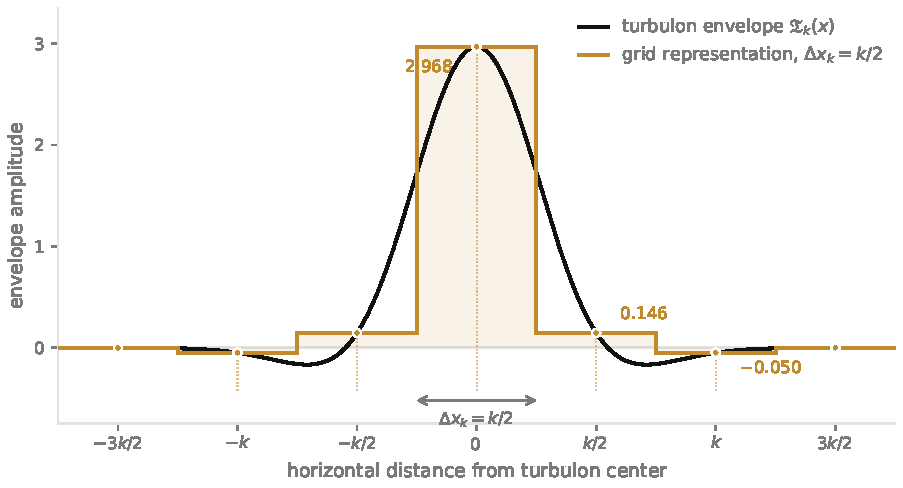
\includegraphics[width=12cm]{concept-figs/s1_working_grid_resolution.pdf}
\caption{One-dimensional transect of the turbulon envelope $\mathfrak{T}_\ell$ (Eqn. \ref{apxeq:turbulon shape}) as resolved on its own working grid at the most aggressive sparsity, $s=1$. The leading constant $\delta$ is set to $\delta = 2.9678$ such that the discrete three-dimensional sum is zero. Note that the three-dimensional sum remains zero even as the sum of the one-dimensional transect shown here is positive.} \label{fig:discretized turbulon}
\end{figure*}

We use horizontally periodic boundary conditions, and along the vertical direction we use zero-padded convolutions while requiring that no turbulons are centered below the surface or above the domain top. [CLAUDE: The implemented exclusion is stronger: no centers within $m\, \ell_z(\ell)$ of the surface or the domain top, with $m$ an input defaulting to 1 --- a full local turbulon depth of standoff per class, not merely non-negative $z$.] Physically, this means that turbulons near the Earth's surface may be ``cut off'' by the boundary but are otherwise unaffected. However, the statistics of $h$ and $q$ near the surface remain affected in a non-obvious way. Without a domain boundary at the surface, there would be turbulons centered at negative values of $z$ that affect $h$ and $q$ at positive $z$ given that some portion of such turbulons might extend to positive $z$. Imposing a boundary at the surface removes the influence of such turbulons and therefore the overall fields $h$ and $q$ are affected. It remains to be determined whether such an effect is physically realistic.


\subsection{Recovering diagnostic variables from prognostic variables}

Once three-dimensional fields of $h(\mathbf{r})$ and $q_t(\mathbf{r})$ are obtained, we recover temperature and water phase at each grid point. We assume the surface pressure $p_s$ is known and use the hypsometric equation to diagnose the pressure at each level; for the simulations described in the main text, $p_s$ is taken from the corresponding host model.

For each column $(x, y)$, we proceed upward from $z = z_{\min}$. At each level, we first test for saturation by assuming all water is in vapor phase, giving a tentative temperature
%
\begin{equation}
    T_{\mathrm{dry}} = \frac{h - L_v q_t - gz}{c_p}. \label{eq:Tdry}
\end{equation}
%
We then compute the saturation mixing ratio $q_{v,\mathrm{sat}}(T_{\mathrm{dry}}, p)$ using Bolton's (1980) formula for the saturation vapor pressure over liquid water,
%
\begin{equation}
    e_s(T) = 611.2 \exp\!\left(\frac{17.67\,(T - 273.15)}{T - 29.65}\right), \label{eq:bolton}
\end{equation}
%
and
%
\begin{equation}
    q_{v,\mathrm{sat}} = \frac{0.622\, e_s}{p - e_s}. \label{eq:qvsat}
\end{equation}
If $q_t \leq q_{v,\mathrm{sat}}(T_{\mathrm{dry}}, p)$, the grid cell is unsaturated: $T = T_{\mathrm{dry}}$, $q_v = q_t$, and $q_c = q_i = 0$.
If $q_t > q_{v,\mathrm{sat}}(T_{\mathrm{dry}}, p)$, condensation has occurred and the temperature must account for latent heat release. We solve
%
\begin{equation}
    h = c_p T + gz + L_v\, q_{v,\mathrm{sat}}(T, p) \label{eq:h_saturated}
\end{equation}
%
for $T$ using Newton's method. Defining $f(T) = c_p T + L_v\, q_{v,\mathrm{sat}}(T, p) + gz - h$, the derivative is
%
\begin{equation}
    f'(T) = c_p + L_v \frac{dq_{v,\mathrm{sat}}}{dT}. \label{eq:fprime}
\end{equation}
%
Differentiating Eqns.~\ref{eq:bolton}--\ref{eq:qvsat},
\begin{align}
    &\frac{de_s}{dT} = \frac{4302.6\, e_s(T)}{(T - 29.65)^2}, \label{eq:des_dT} \\
    &\frac{dq_{v,\mathrm{sat}}}{dT} = \frac{0.622\, p}{(p - e_s)^2} \frac{de_s}{dT}. \label{eq:dqvsat_dT}
\end{align}
%
Thus,
%
\begin{equation}
    f'(T) = c_p + \frac{0.622\, L_v\, p}{(p - e_s)^2} \cdot \frac{4302.6\, e_s(T)}{(T - 29.65)^2}. \label{eq:fprime_explicit}
\end{equation}
%%%%%%%%%%%%%%%%%%%%%%%%%%%%%%%%%%%%%%%%%%%%%%%%%%%%%%%%%%%%%%%%%%%
% MATHEMATICA VERIFICATION
%%%%%%%%%%%%%%%%%%%%%%%%%%%%%%%%%%%%%%%%%%%%%%%%%%%%%%%%%%%%%%%%%%%

% cp = 1004;
% Lv = 2.5*10^6;
% g = 9.81;
% z = 5000;
% h = 340000;
% es[T_] := 611.2 Exp[17.67 (T - 273.15)/(T - 29.65)]
% qvsat[T_, p_] := 0.622 es[T]/(p - es[T])

% f[T_, p_] := 1004 T + 2.5*10^6 qvsat[T, p] + 9.81*5000 - 340000

% fprime[T_, p_] := 
%  1004 + 0.622*2.5*10^6*p/(p - es[T])^2*4302.6 es[T]/(T - 29.65)^2

% (*Numerical derivative*)
% fprimeNum[T_, p_] := (f[T + 0.001, p] - f[T - 0.001, p])/0.002

% (*Test across reasonable T and p*)
% Table[{T, p, fprime[T, p], 
%     fprimeNum[T, p], (fprime[T, p] - fprimeNum[T, p])/
%      fprimeNum[T, p]}, {T, 240, 300, 
%     10}, {p, {50000, 80000, 101325}}] // Flatten[#, 1] & // TableForm
%%%%%%%%%%%%%%%%%%%%%%%%%%%%%%%%%%%%%%%%%%%%%%%%%%%%%%%%%%%%%%%%%%%
%%%%%%%%%%%%%%%%%%%%%%%%%%%%%%%%%%%%%%%%%%%%%%%%%%%%%%%%%%%%%%%%%%%
The unsaturated temperature $T_{\mathrm{dry}}$ serves as the initial guess, and a fixed five Newton iterations are performed, which is ample for convergence from this starting point. The vapor mixing ratio is then $q_v = q_{v,\mathrm{sat}}(T, p)$ and the total condensate is $q_t - q_v$, which is partitioned into liquid and ice as
%
\begin{equation}
    q_c = \omega\,(q_t - q_v), \quad q_i = (1 - \omega)\,(q_t - q_v), \label{eq:phase_partition}
\end{equation}
%
where
%
\begin{equation}
    \omega = \max\!\Big(0,\, \min\!\Big(1,\, \frac{T - 235.15}{273.15 - 235.15}\Big)\Big) \label{eq:liquid fraction}
\end{equation}
%
following \citet{khairoutdinov2003}. Finally, the pressure at the next level is computed using the hypsometric equation,
%
\begin{equation}
    p(z + \Delta z) = p(z) \exp\!\left(\frac{-g\,\Delta z}{R_d\, T_v}\right), \label{eq:hypsometric}
\end{equation}
%
where $T_v = T(1 + 0.608\, q_v)$ is the virtual temperature.


\section{Cloud aspect ratio scaling from \citet{guillaume2018}} \label{sec:guillame}

The study by \citet{guillaume2018} measured distributions of cloud chord lengths along the horizontal and vertical directions. Although they did not directly report cloud aspect ratios as a function of size, their reported size distribution exponents are algebraically equivalent. Note that a similar argument is provided by (CITE LOVEJOYS NOTE)

Specifically, we seek a function of the form 
\begin{align}
  h \propto w^{H_z}\label{fhdjkalbfuke}
\end{align}
where $h$ is cloud height, $w$ is cloud width, and $H_z$ is the unknown scaling exponent relating the two. Here, cloud widths and heights are understood as average values, and Eqn. \ref{fhdjkalbfuke} does not necessarily apply to every individual cloud. 

\citet{guillaume2018} instead reported size distribution exponents for the distributions for $h$ and $w$, which also represent statistical properties computed over many clouds. They found, over an intermediate scale invariant range, probability density functions followed
\begin{align}
  \frac{dn}{dw}\propto w^{-1.66} \\
  \frac{dn}{dh}\propto h^{-2.23},
\end{align}
which coorespond to cumulative distribution functions
\begin{align}
  n(w)\propto w^{-0.66} \\
  n(h) \propto h^{-1.23}.
\end{align}
To relate these cumulative size distribution exponents to Eqn. \ref{fhdjkalbfuke}, first note that Eqn. \ref{fhdjkalbfuke} implies 
$$H_z=d\log h/d\log w.$$
Taking logarithms of the cumulative distribution functions gives
\begin{align}
  \log n = -0.66\log w +\text{const.}\\
  \log n = -1.23 \log h +\text{const.}.
\end{align}
Differentiating to eliminate the constant and then solving for $d\log h/d\log w$, we obtain
\begin{align}
  H_z = \frac{0.66}{1.23} = 0.54,
\end{align}
which is extremely close to the theoretical value $5/9=0.55\dots$ proposed by \citet{schertzer1985}.

\section{Renderings for larger domains containing deep convection}

For the other case, we use the same nesting approach but start with the large-domain square simulations used for the MODIS comparison in Sect. (REF). These simulations proceed in two steps, first simulating a centered nest of size X by X, with a X grid spacing and a grid size of XxXxX. A secondary centered nest is then simulated in the lowest X km vertically, spanning XxX horizontally for a grid of size XxXxX and a horizontal grid spacing of X~m.

% \noappendix       %% use this to mark the end of the appendix section. Otherwise the figures might be numbered incorrectly (e.g. 10 instead of 1).

%% Regarding figures and tables in appendices, the following two options are possible depending on your general handling of figures and tables in the manuscript environment:

%% Option 1: If you sorted all figures and tables into the sections of the text, please also sort the appendix figures and appendix tables into the respective appendix sections.
%% They will be correctly named automatically.

%% Option 2: If you put all figures after the reference list, please insert appendix tables and figures after the normal tables and figures.
%% To rename them correctly to A1, A2, etc., please add the following commands in front of them:

% \appendixfigures  %% needs to be added in front of appendix figures

% \appendixtables   %% needs to be added in front of appendix tables

%% Please add \clearpage between each table and/or figure. Further guidelines on figures and tables can be found below.



% \authorcontribution{TEXT} %% this section is mandatory

% \competinginterests{TEXT} %% this section is mandatory even if you declare that no competing interests are present

% \disclaimer{TEXT} %% optional section

% \begin{acknowledgements}
% TEXT
% \end{acknowledgements}




%% REFERENCES


%% Since the Copernicus LaTeX package includes the BibTeX style file copernicus.bst,
%% authors experienced with BibTeX only have to include the following two lines:
%%
\bibliographystyle{copernicus}
\bibliography{sources.bib}
%%
%% URLs and DOIs can be entered in your BibTeX file as:
%%
%% URL = {http://www.xyz.org/~jones/idx_g.htm}
%% DOI = {10.5194/xyz}


%% LITERATURE CITATIONS
%%
%% command                        & example result
%% \citet{jones90}|               & Jones et al. (1990)
%% \citep{jones90}|               & (Jones et al., 1990)
%% \citep{jones90,jones93}|       & (Jones et al., 1990, 1993)
%% \citep[p.~32]{jones90}|        & (Jones et al., 1990, p.~32)
%% \citep[e.g.,][]{jones90}|      & (e.g., Jones et al., 1990)
%% \citep[e.g.,][p.~32]{jones90}| & (e.g., Jones et al., 1990, p.~32)
%% \citeauthor{jones90}|          & Jones et al.
%% \citeyear{jones90}|            & 1990



%% FIGURES

%% When figures and tables are placed at the end of the MS (article in one-column style), please add \clearpage
%% between bibliography and first table and/or figure as well as between each table and/or figure.

% The figure files should be labelled correctly with Arabic numerals (e.g. fig01.jpg, fig02.png).


%% ONE-COLUMN FIGURES

%%f
%\begin{figure}[t]
%\includegraphics[width=8.3cm]{FILE NAME}
%\caption{TEXT}
%\end{figure}
%
%%% TWO-COLUMN FIGURES
%
%%f
%\begin{figure*}[t]
%\includegraphics[width=12cm]{FILE NAME}
%\caption{TEXT}
%\end{figure*}
%
%
%%% TABLES
%%%
%%% The different columns must be seperated with a & command and should
%%% end with \\ to identify the column brake.
%
%%% ONE-COLUMN TABLE
%
%%t
%\begin{table}[t]
%\caption{TEXT}
%\begin{tabular}{column = lcr}
%\tophline
%
%\middlehline
%
%\bottomhline
%\end{tabular}
%\belowtable{} % Table Footnotes
%\end{table}
%
%%% TWO-COLUMN TABLE
%
%%t
%\begin{table*}[t]
%\caption{TEXT}
%\begin{tabular}{column = lcr}
%\tophline
%
%\middlehline
%
%\bottomhline
%\end{tabular}
%\belowtable{} % Table Footnotes
%\end{table*}
%
%%% LANDSCAPE TABLE
%
%%t
%\begin{sidewaystable*}[t]
%\caption{TEXT}
%\begin{tabular}{column = lcr}
%\tophline
%
%\middlehline
%
%\bottomhline
%\end{tabular}
%\belowtable{} % Table Footnotes
%\end{sidewaystable*}
%
%
%%% MATHEMATICAL EXPRESSIONS
%
%%% All papers typeset by Copernicus Publications follow the math typesetting regulations
%%% given by the IUPAC Green Book (IUPAC: Quantities, Units and Symbols in Physical Chemistry,
%%% 2nd Edn., Blackwell Science, available at: http://old.iupac.org/publications/books/gbook/green_book_2ed.pdf, 1993).
%%%
%%% Physical quantities/variables are typeset in italic font (t for time, T for Temperature)
%%% Indices which are not defined are typeset in italic font (x, y, z, a, b, c)
%%% Items/objects which are defined are typeset in roman font (Car A, Car B)
%%% Descriptions/specifications which are defined by itself are typeset in roman font (abs, rel, ref, tot, net, ice)
%%% Abbreviations from 2 letters are typeset in roman font (RH, LAI)
%%% Vectors are identified in bold italic font using \vec{x}
%%% Matrices are identified in bold roman font
%%% Multiplication signs are typeset using the LaTeX commands \times (for vector products, grids, and exponential notations) or \cdot
%%% The character * should not be applied as mutliplication sign
%
%
%%% EQUATIONS
%
%%% Single-row equation
%
%\begin{equation}
%
%\end{equation}
%
%%% Multiline equation
%
%\begin{align}
%& 3 + 5 = 8\\
%& 3 + 5 = 8\\
%& 3 + 5 = 8
%\end{align}
%
%
%%% MATRICES
%
%\begin{matrix}
%x & y & z\\
%x & y & z\\
%x & y & z\\
%\end{matrix}
%
%
%%% ALGORITHM
%
%\begin{algorithm}
%\caption{...}
%\label{a1}
%\begin{algorithmic}
%...
%\end{algorithmic}
%\end{algorithm}
%
%
%%% CHEMICAL FORMULAS AND REACTIONS
%
%%% For formulas embedded in the text, please use \chem{}
%
%%% The reaction environment creates labels including the letter R, i.e. (R1), (R2), etc.
%
%\begin{reaction}
%%% \rightarrow should be used for normal (one-way) chemical reactions
%%% \rightleftharpoons should be used for equilibria
%%% \leftrightarrow should be used for resonance structures
%\end{reaction}
%
%
%%% PHYSICAL UNITS
%%%
%%% Please use \unit{} and apply the exponential notation


\end{document}
